% **************************************************************************************************************
% A Classic Thesis Style
% An Homage to The Elements of Typographic Style
%
% Copyright (C) 2017 André Miede and Ivo Pletikosić
%
% If you like the style then I would appreciate a postcard. My address
% can be found in the file ClassicThesis.pdf. A collection of the
% postcards I received so far is available online at
% http://postcards.miede.de
%
% License:
% This program is free software; you can redistribute it and/or modify
% it under the terms of the GNU General Public License as published by
% the Free Software Foundation; either version 2 of the License, or
% (at your option) any later version.
%
% This program is distributed in the hope that it will be useful,
% but WITHOUT ANY WARRANTY; without even the implied warranty of
% MERCHANTABILITY or FITNESS FOR A PARTICULAR PURPOSE.  See the
% GNU General Public License for more details.
%
% You should have received a copy of the GNU General Public License
% along with this program; see the file COPYING.  If not, write to
% the Free Software Foundation, Inc., 59 Temple Place - Suite 330,
% Boston, MA 02111-1307, USA.
%
% PLEASE SEE ALSO THE AUTHORS' NOTE REGARDING THIS LICENSE
% IN THE DOCUMENTATION (ClassicThesis.pdf --> Chapter 1 / Chapter01.tex)
% **************************************************************************************************************
\RequirePackage{silence} % :-\
    \WarningFilter{scrreprt}{Usage of package `titlesec'}
    \WarningFilter{titlesec}{Non standard sectioning command detected}
\documentclass[ twoside,openright,titlepage,numbers=noenddot,headinclude,%1headlines,% letterpaper a4paper
                footinclude=true,cleardoublepage=empty,abstractoff, % <--- obsolete, remove (todo)
                BCOR=5mm,paper=a4,fontsize=11pt,%11pt,a4paper,%
                american,%
                ]{scrreprt}

%********************************************************************
% Note: Make all your adjustments in here
%*******************************************************
% ****************************************************************************************************
% classicthesis-config.tex
% formerly known as loadpackages.sty, classicthesis-ldpkg.sty, and classicthesis-preamble.sty
% Use it at the beginning of your ClassicThesis.tex, or as a LaTeX Preamble
% in your ClassicThesis.{tex,lyx} with % ****************************************************************************************************
% classicthesis-config.tex
% formerly known as loadpackages.sty, classicthesis-ldpkg.sty, and classicthesis-preamble.sty
% Use it at the beginning of your ClassicThesis.tex, or as a LaTeX Preamble
% in your ClassicThesis.{tex,lyx} with % ****************************************************************************************************
% classicthesis-config.tex
% formerly known as loadpackages.sty, classicthesis-ldpkg.sty, and classicthesis-preamble.sty
% Use it at the beginning of your ClassicThesis.tex, or as a LaTeX Preamble
% in your ClassicThesis.{tex,lyx} with \input{classicthesis-config}
% ****************************************************************************************************
% If you like the classicthesis, then I would appreciate a postcard.
% My address can be found in the file ClassicThesis.pdf. A collection
% of the postcards I received so far is available online at
% http://postcards.miede.de
% ****************************************************************************************************


% ****************************************************************************************************
% 0. Set the encoding of your files. UTF-8 is the only sensible encoding nowadays. If you can't read
% äöüßáéçèê∂åëæƒÏ€ then change the encoding setting in your editor, not the line below. If your editor
% does not support utf8 use another editor!
% ****************************************************************************************************

\PassOptionsToPackage{utf8}{inputenc}
  \usepackage{inputenc}

% ****************************************************************************************************
% 1. Configure classicthesis for your needs here, e.g., remove "drafting" below
% in order to deactivate the time-stamp on the pages
% (see ClassicThesis.pdf for more information):
% ****************************************************************************************************
\PassOptionsToPackage{
  drafting=false,    % print version information on the bottom of the pages
  tocaligned=false, % the left column of the toc will be aligned (no indentation)
  dottedtoc=false,  % page numbers in ToC flushed right
  parts=true,       % use part division
  eulerchapternumbers=true, % use AMS Euler for chapter font (otherwise Palatino)
  linedheaders=false,       % chaper headers will have line above and beneath
  floatperchapter=true,     % numbering per chapter for all floats (i.e., Figure 1.1)
  listings=true,    % load listings package and setup LoL
  subfig=true,      % setup for preloaded subfig package
  eulermath=false,  % use awesome Euler fonts for mathematical formulae (only with pdfLaTeX)
  beramono=true,    % toggle a nice monospaced font (w/ bold)
  minionpro=false   % setup for minion pro font; use minion pro small caps as well (only with pdfLaTeX)
}{classicthesis}


% ****************************************************************************************************
% 2. Personal data and user ad-hoc commands
% ****************************************************************************************************
\newcommand{\myTitle}{Constrained Clustering\xspace}
\newcommand{\mySubtitle}{A Metaheuristic Approach\xspace}
\newcommand{\myDegree}{Master's Degree in Data Science and Computer Engineering\xspace}
\newcommand{\myName}{Germán González Almagro\xspace}
\newcommand{\myProf}{Salvador García López\xspace}
%\newcommand{\myOtherProf}{Juan José Escobar Pérez\xspace}
\newcommand{\mySupervisor}{Put name here\xspace}
\newcommand{\myFaculty}{Escuela Técnica Superior de Ingenierías Informática y de Telecomunicación\xspace}
\newcommand{\myOtherFaculty}{Escuela Internacional de Posgrado de la Universidad de Granada\xspace}
\newcommand{\myDepartment}{Department of Computer Science and Artificial Intelligence\xspace}
\newcommand{\myUni}{University of Granada\xspace}
\newcommand{\myLocation}{Granada\xspace}
\newcommand{\myTime}{July 2019\xspace}
\newcommand{\myVersion}{version 0.1}

% ********************************************************************
% Setup, finetuning, and useful commands
% ********************************************************************
\newcounter{dummy} % necessary for correct hyperlinks (to index, bib, etc.)
\newlength{\abcd} % for ab..z string length calculation
\providecommand{\mLyX}{L\kern-.1667em\lower.25em\hbox{Y}\kern-.125emX\@}
\newcommand{\ie}{i.\,e.}
\newcommand{\Ie}{I.\,e.}
\newcommand{\eg}{e.\,g.}
\newcommand{\Eg}{E.\,g.}
% ****************************************************************************************************


% ****************************************************************************************************
% 3. Loading some handy packages
% ****************************************************************************************************
\usepackage{varwidth}
\usepackage[ruled, lined, onelanguage, linesnumbered]{algorithm2e}
\SetKwProg{Fn}{Function}{}{end}
\SetKwProg{Proc}{Procedure}{}{end}
\usepackage{fixltx2e}
% ********************************************************************
% Packages with options that might require adjustments
% ********************************************************************
%\PassOptionsToPackage{ngerman,american}{babel}   % change this to your language(s), main language last
% Spanish languages need extra options in order to work with this template
%\PassOptionsToPackage{spanish,es-lcroman}{babel}
    \usepackage{babel}

\usepackage{csquotes}
\PassOptionsToPackage{%
  %backend=biber,bibencoding=utf8, %instead of bibtex
  backend=bibtex8,bibencoding=ascii,%
  language=auto,%
  style=numeric-comp,%
  %style=authoryear-comp, % Author 1999, 2010
  %bibstyle=authoryear,dashed=false, % dashed: substitute rep. author with ---
  sorting=none, % name, year, title
  maxbibnames=10, % default: 3, et al.
  %backref=true,%
  natbib=true % natbib compatibility mode (\citep and \citet still work)
}{biblatex}
    \usepackage{biblatex}

\PassOptionsToPackage{fleqn}{amsmath}       % math environments and more by the AMS
  \usepackage{amsmath}

% ********************************************************************
% General useful packages
% ********************************************************************
\PassOptionsToPackage{T1}{fontenc} % T2A for cyrillics
  \usepackage{fontenc}
\usepackage{textcomp} % fix warning with missing font shapes
\usepackage{scrhack} % fix warnings when using KOMA with listings package
\usepackage{xspace} % to get the spacing after macros right
\usepackage{mparhack} % get marginpar right
%\usepackage{fixltx2e} % fixes some LaTeX stuff --> since 2015 in the LaTeX kernel (see below)
% \usepackage[latest]{latexrelease} % emulate newer kernel version if older is detected
\PassOptionsToPackage{printonlyused,smaller}{acronym}
  \usepackage{acronym} % nice macros for handling all acronyms in the thesis
  %\renewcommand{\bflabel}[1]{{#1}\hfill} % fix the list of acronyms --> no longer working
  %\renewcommand*{\acsfont}[1]{\textsc{#1}}
  %\renewcommand*{\aclabelfont}[1]{\acsfont{#1}}
  %\def\bflabel#1{{#1\hfill}}
  \def\bflabel#1{{\acsfont{#1}\hfill}}
  \def\aclabelfont#1{\acsfont{#1}}
% ****************************************************************************************************
%\usepackage{pgfplots} % External TikZ/PGF support (thanks to Andreas Nautsch)
%\usetikzlibrary{external}
%\tikzexternalize[mode=list and make, prefix=ext-tikz/]
% ****************************************************************************************************


% ****************************************************************************************************
% 4. Setup floats: tables, (sub)figures, and captions
% ****************************************************************************************************
\usepackage{tabularx} % better tables
  \setlength{\extrarowheight}{3pt} % increase table row height
\newcommand{\tableheadline}[1]{\multicolumn{1}{c}{\spacedlowsmallcaps{#1}}}
\newcommand{\myfloatalign}{\centering} % to be used with each float for alignment
\usepackage{caption}
% Thanks to cgnieder and Claus Lahiri
% http://tex.stackexchange.com/questions/69349/spacedlowsmallcaps-in-caption-label
% [REMOVED DUE TO OTHER PROBLEMS, SEE ISSUE #82]
%\DeclareCaptionLabelFormat{smallcaps}{\bothIfFirst{#1}{~}\MakeTextLowercase{\textsc{#2}}}
%\captionsetup{font=small,labelformat=smallcaps} % format=hang,
\captionsetup{font=small} % format=hang,
\usepackage{subfig}
% ****************************************************************************************************


% ****************************************************************************************************
% 5. Setup code listings
% ****************************************************************************************************
\usepackage{listings}
%\lstset{emph={trueIndex,root},emphstyle=\color{BlueViolet}}%\underbar} % for special keywords
\lstset{language=[LaTeX]Tex,%C++,
  morekeywords={PassOptionsToPackage,selectlanguage},
  keywordstyle=\color{RoyalBlue},%\bfseries,
  basicstyle=\small\ttfamily,
  %identifierstyle=\color{NavyBlue},
  commentstyle=\color{Green}\ttfamily,
  stringstyle=\rmfamily,
  numbers=none,%left,%
  numberstyle=\scriptsize,%\tiny
  stepnumber=5,
  numbersep=8pt,
  showstringspaces=false,
  breaklines=true,
  %frameround=ftff,
  %frame=single,
  belowcaptionskip=.75\baselineskip
  %frame=L
}
% ****************************************************************************************************


% ****************************************************************************************************
% 6. PDFLaTeX, hyperreferences, and citation backreferences
% ****************************************************************************************************
% ********************************************************************
% Using PDFLaTeX
% ********************************************************************
\PassOptionsToPackage{hyperfootnotes=false,pdfpagelabels}{hyperref}
  \usepackage{hyperref}  % backref linktocpage pagebackref
%\ifpdf
%\pdfcompresslevel=9
%\pdfadjustspacing=1
%\fi
%\PassOptionsToPackage{pdftex}{graphicx} %%%IVO: driver will be chosen automatically
  \usepackage{graphicx}


% ********************************************************************
% Hyperreferences
% ********************************************************************
\hypersetup{%
  %draft, % hyperref's draft mode, for printing see below
  colorlinks=true, linktocpage=true, pdfstartpage=3, pdfstartview=FitV,%
  % uncomment the following line if you want to have black links (e.g., for printing)
  %colorlinks=false, linktocpage=false, pdfstartpage=3, pdfstartview=FitV, pdfborder={0 0 0},%
  breaklinks=true, pdfpagemode=UseNone, pageanchor=true, pdfpagemode=UseOutlines,%
  plainpages=false, bookmarksnumbered, bookmarksopen=true, bookmarksopenlevel=1,%
  hypertexnames=true, pdfhighlight=/O,%nesting=true,%frenchlinks,%
  %urlcolor=blue, linkcolor=RoyalBlue, citecolor=webgreen, %pagecolor=RoyalBlue,%
  urlcolor=Black, linkcolor=Black, citecolor=Black, %pagecolor=Black,%
  pdftitle={\myTitle},%
  pdfauthor={\textcopyright\ \myName, \myUni, \myFaculty},%
  pdfsubject={},%
  pdfkeywords={},%
  pdfcreator={pdfLaTeX},%
  pdfproducer={LaTeX with hyperref and classicthesis}%
}

% ********************************************************************
% Setup autoreferences
% ********************************************************************
% There are some issues regarding autorefnames
% http://www.ureader.de/msg/136221647.aspx
% http://www.tex.ac.uk/cgi-bin/texfaq2html?label=latexwords
% you have to redefine the makros for the
% language you use, e.g., american, ngerman
% (as chosen when loading babel/AtBeginDocument)
% ********************************************************************
\makeatletter
\@ifpackageloaded{babel}%
  {%
    \addto\extrasamerican{%
      \renewcommand*{\figureautorefname}{Figure}%
      \renewcommand*{\tableautorefname}{Table}%
      \renewcommand*{\partautorefname}{Part}%
      \renewcommand*{\chapterautorefname}{Chapter}%
      \renewcommand*{\sectionautorefname}{Section}%
      \renewcommand*{\subsectionautorefname}{Section}%
      \renewcommand*{\subsubsectionautorefname}{Section}%
    }%
    \addto\extrasngerman{%
      \renewcommand*{\paragraphautorefname}{Absatz}%
      \renewcommand*{\subparagraphautorefname}{Unterabsatz}%
      \renewcommand*{\footnoteautorefname}{Fu\"snote}%
      \renewcommand*{\FancyVerbLineautorefname}{Zeile}%
      \renewcommand*{\theoremautorefname}{Theorem}%
      \renewcommand*{\appendixautorefname}{Anhang}%
      \renewcommand*{\equationautorefname}{Gleichung}%
      \renewcommand*{\itemautorefname}{Punkt}%
    }%
      % Fix to getting autorefs for subfigures right (thanks to Belinda Vogt for changing the definition)
      \providecommand{\subfigureautorefname}{\figureautorefname}%
    }{\relax}
\makeatother


% ****************************************************************************************************
% 7. Last calls before the bar closes
% ****************************************************************************************************
% ********************************************************************
% Development Stuff
% ********************************************************************
\listfiles
%\PassOptionsToPackage{l2tabu,orthodox,abort}{nag}
%  \usepackage{nag}
%\PassOptionsToPackage{warning, all}{onlyamsmath}
%  \usepackage{onlyamsmath}

% ********************************************************************
% Last, but not least...
% ********************************************************************
\usepackage[dottedtoc]{classicthesis}
% ****************************************************************************************************


% ****************************************************************************************************
% 8. Further adjustments (experimental)
% ****************************************************************************************************
% ********************************************************************
% Changing the text area
% ********************************************************************
%\areaset[current]{312pt}{761pt} % 686 (factor 2.2) + 33 head + 42 head \the\footskip
%\setlength{\marginparwidth}{7em}%
%\setlength{\marginparsep}{2em}%

% ********************************************************************
% Using different fonts
% ********************************************************************
%\usepackage[oldstylenums]{kpfonts} % oldstyle notextcomp
%\usepackage[osf]{libertine}
%\usepackage[light,condensed,math]{iwona}
%\renewcommand{\sfdefault}{iwona}
%\usepackage{lmodern} % <-- no osf support :-(
%\usepackage{cfr-lm} %
%\usepackage[urw-garamond]{mathdesign} <-- no osf support :-(
%\usepackage[default,osfigures]{opensans} % scale=0.95
%\usepackage[sfdefault]{FiraSans}
% ********************************************************************
% \usepackage[largesc,osf]{newpxtext}
% Used to fix these:
% https://bitbucket.org/amiede/classicthesis/issues/139/italics-in-pallatino-capitals-chapter
% https://bitbucket.org/amiede/classicthesis/issues/45/problema-testatine-su-classicthesis-style
% ********************************************************************
%\linespread{1.05} % a bit more for Palatino
% ****************************************************************************************************
% ****************************************************************************************************
% If you like the classicthesis, then I would appreciate a postcard.
% My address can be found in the file ClassicThesis.pdf. A collection
% of the postcards I received so far is available online at
% http://postcards.miede.de
% ****************************************************************************************************


% ****************************************************************************************************
% 0. Set the encoding of your files. UTF-8 is the only sensible encoding nowadays. If you can't read
% äöüßáéçèê∂åëæƒÏ€ then change the encoding setting in your editor, not the line below. If your editor
% does not support utf8 use another editor!
% ****************************************************************************************************

\PassOptionsToPackage{utf8}{inputenc}
  \usepackage{inputenc}

% ****************************************************************************************************
% 1. Configure classicthesis for your needs here, e.g., remove "drafting" below
% in order to deactivate the time-stamp on the pages
% (see ClassicThesis.pdf for more information):
% ****************************************************************************************************
\PassOptionsToPackage{
  drafting=false,    % print version information on the bottom of the pages
  tocaligned=false, % the left column of the toc will be aligned (no indentation)
  dottedtoc=false,  % page numbers in ToC flushed right
  parts=true,       % use part division
  eulerchapternumbers=true, % use AMS Euler for chapter font (otherwise Palatino)
  linedheaders=false,       % chaper headers will have line above and beneath
  floatperchapter=true,     % numbering per chapter for all floats (i.e., Figure 1.1)
  listings=true,    % load listings package and setup LoL
  subfig=true,      % setup for preloaded subfig package
  eulermath=false,  % use awesome Euler fonts for mathematical formulae (only with pdfLaTeX)
  beramono=true,    % toggle a nice monospaced font (w/ bold)
  minionpro=false   % setup for minion pro font; use minion pro small caps as well (only with pdfLaTeX)
}{classicthesis}


% ****************************************************************************************************
% 2. Personal data and user ad-hoc commands
% ****************************************************************************************************
\newcommand{\myTitle}{Constrained Clustering\xspace}
\newcommand{\mySubtitle}{A Metaheuristic Approach\xspace}
\newcommand{\myDegree}{Master's Degree in Data Science and Computer Engineering\xspace}
\newcommand{\myName}{Germán González Almagro\xspace}
\newcommand{\myProf}{Salvador García López\xspace}
%\newcommand{\myOtherProf}{Juan José Escobar Pérez\xspace}
\newcommand{\mySupervisor}{Put name here\xspace}
\newcommand{\myFaculty}{Escuela Técnica Superior de Ingenierías Informática y de Telecomunicación\xspace}
\newcommand{\myOtherFaculty}{Escuela Internacional de Posgrado de la Universidad de Granada\xspace}
\newcommand{\myDepartment}{Department of Computer Science and Artificial Intelligence\xspace}
\newcommand{\myUni}{University of Granada\xspace}
\newcommand{\myLocation}{Granada\xspace}
\newcommand{\myTime}{July 2019\xspace}
\newcommand{\myVersion}{version 0.1}

% ********************************************************************
% Setup, finetuning, and useful commands
% ********************************************************************
\newcounter{dummy} % necessary for correct hyperlinks (to index, bib, etc.)
\newlength{\abcd} % for ab..z string length calculation
\providecommand{\mLyX}{L\kern-.1667em\lower.25em\hbox{Y}\kern-.125emX\@}
\newcommand{\ie}{i.\,e.}
\newcommand{\Ie}{I.\,e.}
\newcommand{\eg}{e.\,g.}
\newcommand{\Eg}{E.\,g.}
% ****************************************************************************************************


% ****************************************************************************************************
% 3. Loading some handy packages
% ****************************************************************************************************
\usepackage{varwidth}
\usepackage[ruled, lined, onelanguage, linesnumbered]{algorithm2e}
\SetKwProg{Fn}{Function}{}{end}
\SetKwProg{Proc}{Procedure}{}{end}
\usepackage{fixltx2e}
% ********************************************************************
% Packages with options that might require adjustments
% ********************************************************************
%\PassOptionsToPackage{ngerman,american}{babel}   % change this to your language(s), main language last
% Spanish languages need extra options in order to work with this template
%\PassOptionsToPackage{spanish,es-lcroman}{babel}
    \usepackage{babel}

\usepackage{csquotes}
\PassOptionsToPackage{%
  %backend=biber,bibencoding=utf8, %instead of bibtex
  backend=bibtex8,bibencoding=ascii,%
  language=auto,%
  style=numeric-comp,%
  %style=authoryear-comp, % Author 1999, 2010
  %bibstyle=authoryear,dashed=false, % dashed: substitute rep. author with ---
  sorting=none, % name, year, title
  maxbibnames=10, % default: 3, et al.
  %backref=true,%
  natbib=true % natbib compatibility mode (\citep and \citet still work)
}{biblatex}
    \usepackage{biblatex}

\PassOptionsToPackage{fleqn}{amsmath}       % math environments and more by the AMS
  \usepackage{amsmath}

% ********************************************************************
% General useful packages
% ********************************************************************
\PassOptionsToPackage{T1}{fontenc} % T2A for cyrillics
  \usepackage{fontenc}
\usepackage{textcomp} % fix warning with missing font shapes
\usepackage{scrhack} % fix warnings when using KOMA with listings package
\usepackage{xspace} % to get the spacing after macros right
\usepackage{mparhack} % get marginpar right
%\usepackage{fixltx2e} % fixes some LaTeX stuff --> since 2015 in the LaTeX kernel (see below)
% \usepackage[latest]{latexrelease} % emulate newer kernel version if older is detected
\PassOptionsToPackage{printonlyused,smaller}{acronym}
  \usepackage{acronym} % nice macros for handling all acronyms in the thesis
  %\renewcommand{\bflabel}[1]{{#1}\hfill} % fix the list of acronyms --> no longer working
  %\renewcommand*{\acsfont}[1]{\textsc{#1}}
  %\renewcommand*{\aclabelfont}[1]{\acsfont{#1}}
  %\def\bflabel#1{{#1\hfill}}
  \def\bflabel#1{{\acsfont{#1}\hfill}}
  \def\aclabelfont#1{\acsfont{#1}}
% ****************************************************************************************************
%\usepackage{pgfplots} % External TikZ/PGF support (thanks to Andreas Nautsch)
%\usetikzlibrary{external}
%\tikzexternalize[mode=list and make, prefix=ext-tikz/]
% ****************************************************************************************************


% ****************************************************************************************************
% 4. Setup floats: tables, (sub)figures, and captions
% ****************************************************************************************************
\usepackage{tabularx} % better tables
  \setlength{\extrarowheight}{3pt} % increase table row height
\newcommand{\tableheadline}[1]{\multicolumn{1}{c}{\spacedlowsmallcaps{#1}}}
\newcommand{\myfloatalign}{\centering} % to be used with each float for alignment
\usepackage{caption}
% Thanks to cgnieder and Claus Lahiri
% http://tex.stackexchange.com/questions/69349/spacedlowsmallcaps-in-caption-label
% [REMOVED DUE TO OTHER PROBLEMS, SEE ISSUE #82]
%\DeclareCaptionLabelFormat{smallcaps}{\bothIfFirst{#1}{~}\MakeTextLowercase{\textsc{#2}}}
%\captionsetup{font=small,labelformat=smallcaps} % format=hang,
\captionsetup{font=small} % format=hang,
\usepackage{subfig}
% ****************************************************************************************************


% ****************************************************************************************************
% 5. Setup code listings
% ****************************************************************************************************
\usepackage{listings}
%\lstset{emph={trueIndex,root},emphstyle=\color{BlueViolet}}%\underbar} % for special keywords
\lstset{language=[LaTeX]Tex,%C++,
  morekeywords={PassOptionsToPackage,selectlanguage},
  keywordstyle=\color{RoyalBlue},%\bfseries,
  basicstyle=\small\ttfamily,
  %identifierstyle=\color{NavyBlue},
  commentstyle=\color{Green}\ttfamily,
  stringstyle=\rmfamily,
  numbers=none,%left,%
  numberstyle=\scriptsize,%\tiny
  stepnumber=5,
  numbersep=8pt,
  showstringspaces=false,
  breaklines=true,
  %frameround=ftff,
  %frame=single,
  belowcaptionskip=.75\baselineskip
  %frame=L
}
% ****************************************************************************************************


% ****************************************************************************************************
% 6. PDFLaTeX, hyperreferences, and citation backreferences
% ****************************************************************************************************
% ********************************************************************
% Using PDFLaTeX
% ********************************************************************
\PassOptionsToPackage{hyperfootnotes=false,pdfpagelabels}{hyperref}
  \usepackage{hyperref}  % backref linktocpage pagebackref
%\ifpdf
%\pdfcompresslevel=9
%\pdfadjustspacing=1
%\fi
%\PassOptionsToPackage{pdftex}{graphicx} %%%IVO: driver will be chosen automatically
  \usepackage{graphicx}


% ********************************************************************
% Hyperreferences
% ********************************************************************
\hypersetup{%
  %draft, % hyperref's draft mode, for printing see below
  colorlinks=true, linktocpage=true, pdfstartpage=3, pdfstartview=FitV,%
  % uncomment the following line if you want to have black links (e.g., for printing)
  %colorlinks=false, linktocpage=false, pdfstartpage=3, pdfstartview=FitV, pdfborder={0 0 0},%
  breaklinks=true, pdfpagemode=UseNone, pageanchor=true, pdfpagemode=UseOutlines,%
  plainpages=false, bookmarksnumbered, bookmarksopen=true, bookmarksopenlevel=1,%
  hypertexnames=true, pdfhighlight=/O,%nesting=true,%frenchlinks,%
  %urlcolor=blue, linkcolor=RoyalBlue, citecolor=webgreen, %pagecolor=RoyalBlue,%
  urlcolor=Black, linkcolor=Black, citecolor=Black, %pagecolor=Black,%
  pdftitle={\myTitle},%
  pdfauthor={\textcopyright\ \myName, \myUni, \myFaculty},%
  pdfsubject={},%
  pdfkeywords={},%
  pdfcreator={pdfLaTeX},%
  pdfproducer={LaTeX with hyperref and classicthesis}%
}

% ********************************************************************
% Setup autoreferences
% ********************************************************************
% There are some issues regarding autorefnames
% http://www.ureader.de/msg/136221647.aspx
% http://www.tex.ac.uk/cgi-bin/texfaq2html?label=latexwords
% you have to redefine the makros for the
% language you use, e.g., american, ngerman
% (as chosen when loading babel/AtBeginDocument)
% ********************************************************************
\makeatletter
\@ifpackageloaded{babel}%
  {%
    \addto\extrasamerican{%
      \renewcommand*{\figureautorefname}{Figure}%
      \renewcommand*{\tableautorefname}{Table}%
      \renewcommand*{\partautorefname}{Part}%
      \renewcommand*{\chapterautorefname}{Chapter}%
      \renewcommand*{\sectionautorefname}{Section}%
      \renewcommand*{\subsectionautorefname}{Section}%
      \renewcommand*{\subsubsectionautorefname}{Section}%
    }%
    \addto\extrasngerman{%
      \renewcommand*{\paragraphautorefname}{Absatz}%
      \renewcommand*{\subparagraphautorefname}{Unterabsatz}%
      \renewcommand*{\footnoteautorefname}{Fu\"snote}%
      \renewcommand*{\FancyVerbLineautorefname}{Zeile}%
      \renewcommand*{\theoremautorefname}{Theorem}%
      \renewcommand*{\appendixautorefname}{Anhang}%
      \renewcommand*{\equationautorefname}{Gleichung}%
      \renewcommand*{\itemautorefname}{Punkt}%
    }%
      % Fix to getting autorefs for subfigures right (thanks to Belinda Vogt for changing the definition)
      \providecommand{\subfigureautorefname}{\figureautorefname}%
    }{\relax}
\makeatother


% ****************************************************************************************************
% 7. Last calls before the bar closes
% ****************************************************************************************************
% ********************************************************************
% Development Stuff
% ********************************************************************
\listfiles
%\PassOptionsToPackage{l2tabu,orthodox,abort}{nag}
%  \usepackage{nag}
%\PassOptionsToPackage{warning, all}{onlyamsmath}
%  \usepackage{onlyamsmath}

% ********************************************************************
% Last, but not least...
% ********************************************************************
\usepackage[dottedtoc]{classicthesis}
% ****************************************************************************************************


% ****************************************************************************************************
% 8. Further adjustments (experimental)
% ****************************************************************************************************
% ********************************************************************
% Changing the text area
% ********************************************************************
%\areaset[current]{312pt}{761pt} % 686 (factor 2.2) + 33 head + 42 head \the\footskip
%\setlength{\marginparwidth}{7em}%
%\setlength{\marginparsep}{2em}%

% ********************************************************************
% Using different fonts
% ********************************************************************
%\usepackage[oldstylenums]{kpfonts} % oldstyle notextcomp
%\usepackage[osf]{libertine}
%\usepackage[light,condensed,math]{iwona}
%\renewcommand{\sfdefault}{iwona}
%\usepackage{lmodern} % <-- no osf support :-(
%\usepackage{cfr-lm} %
%\usepackage[urw-garamond]{mathdesign} <-- no osf support :-(
%\usepackage[default,osfigures]{opensans} % scale=0.95
%\usepackage[sfdefault]{FiraSans}
% ********************************************************************
% \usepackage[largesc,osf]{newpxtext}
% Used to fix these:
% https://bitbucket.org/amiede/classicthesis/issues/139/italics-in-pallatino-capitals-chapter
% https://bitbucket.org/amiede/classicthesis/issues/45/problema-testatine-su-classicthesis-style
% ********************************************************************
%\linespread{1.05} % a bit more for Palatino
% ****************************************************************************************************
% ****************************************************************************************************
% If you like the classicthesis, then I would appreciate a postcard.
% My address can be found in the file ClassicThesis.pdf. A collection
% of the postcards I received so far is available online at
% http://postcards.miede.de
% ****************************************************************************************************


% ****************************************************************************************************
% 0. Set the encoding of your files. UTF-8 is the only sensible encoding nowadays. If you can't read
% äöüßáéçèê∂åëæƒÏ€ then change the encoding setting in your editor, not the line below. If your editor
% does not support utf8 use another editor!
% ****************************************************************************************************

\PassOptionsToPackage{utf8}{inputenc}
  \usepackage{inputenc}

% ****************************************************************************************************
% 1. Configure classicthesis for your needs here, e.g., remove "drafting" below
% in order to deactivate the time-stamp on the pages
% (see ClassicThesis.pdf for more information):
% ****************************************************************************************************
\PassOptionsToPackage{
  drafting=false,    % print version information on the bottom of the pages
  tocaligned=false, % the left column of the toc will be aligned (no indentation)
  dottedtoc=false,  % page numbers in ToC flushed right
  parts=true,       % use part division
  eulerchapternumbers=true, % use AMS Euler for chapter font (otherwise Palatino)
  linedheaders=false,       % chaper headers will have line above and beneath
  floatperchapter=true,     % numbering per chapter for all floats (i.e., Figure 1.1)
  listings=true,    % load listings package and setup LoL
  subfig=true,      % setup for preloaded subfig package
  eulermath=false,  % use awesome Euler fonts for mathematical formulae (only with pdfLaTeX)
  beramono=true,    % toggle a nice monospaced font (w/ bold)
  minionpro=false   % setup for minion pro font; use minion pro small caps as well (only with pdfLaTeX)
}{classicthesis}


% ****************************************************************************************************
% 2. Personal data and user ad-hoc commands
% ****************************************************************************************************
\newcommand{\myTitle}{Constrained Clustering\xspace}
\newcommand{\mySubtitle}{A Metaheuristic Approach\xspace}
\newcommand{\myDegree}{Master's Degree in Data Science and Computer Engineering\xspace}
\newcommand{\myName}{Germán González Almagro\xspace}
\newcommand{\myProf}{Salvador García López\xspace}
%\newcommand{\myOtherProf}{Juan José Escobar Pérez\xspace}
\newcommand{\mySupervisor}{Put name here\xspace}
\newcommand{\myFaculty}{Escuela Técnica Superior de Ingenierías Informática y de Telecomunicación\xspace}
\newcommand{\myOtherFaculty}{Escuela Internacional de Posgrado de la Universidad de Granada\xspace}
\newcommand{\myDepartment}{Department of Computer Science and Artificial Intelligence\xspace}
\newcommand{\myUni}{University of Granada\xspace}
\newcommand{\myLocation}{Granada\xspace}
\newcommand{\myTime}{July 2019\xspace}
\newcommand{\myVersion}{version 0.1}

% ********************************************************************
% Setup, finetuning, and useful commands
% ********************************************************************
\newcounter{dummy} % necessary for correct hyperlinks (to index, bib, etc.)
\newlength{\abcd} % for ab..z string length calculation
\providecommand{\mLyX}{L\kern-.1667em\lower.25em\hbox{Y}\kern-.125emX\@}
\newcommand{\ie}{i.\,e.}
\newcommand{\Ie}{I.\,e.}
\newcommand{\eg}{e.\,g.}
\newcommand{\Eg}{E.\,g.}
% ****************************************************************************************************


% ****************************************************************************************************
% 3. Loading some handy packages
% ****************************************************************************************************
\usepackage{varwidth}
\usepackage[ruled, lined, onelanguage, linesnumbered]{algorithm2e}
\SetKwProg{Fn}{Function}{}{end}
\SetKwProg{Proc}{Procedure}{}{end}
\usepackage{fixltx2e}
% ********************************************************************
% Packages with options that might require adjustments
% ********************************************************************
%\PassOptionsToPackage{ngerman,american}{babel}   % change this to your language(s), main language last
% Spanish languages need extra options in order to work with this template
%\PassOptionsToPackage{spanish,es-lcroman}{babel}
    \usepackage{babel}

\usepackage{csquotes}
\PassOptionsToPackage{%
  %backend=biber,bibencoding=utf8, %instead of bibtex
  backend=bibtex8,bibencoding=ascii,%
  language=auto,%
  style=numeric-comp,%
  %style=authoryear-comp, % Author 1999, 2010
  %bibstyle=authoryear,dashed=false, % dashed: substitute rep. author with ---
  sorting=none, % name, year, title
  maxbibnames=10, % default: 3, et al.
  %backref=true,%
  natbib=true % natbib compatibility mode (\citep and \citet still work)
}{biblatex}
    \usepackage{biblatex}

\PassOptionsToPackage{fleqn}{amsmath}       % math environments and more by the AMS
  \usepackage{amsmath}

% ********************************************************************
% General useful packages
% ********************************************************************
\PassOptionsToPackage{T1}{fontenc} % T2A for cyrillics
  \usepackage{fontenc}
\usepackage{textcomp} % fix warning with missing font shapes
\usepackage{scrhack} % fix warnings when using KOMA with listings package
\usepackage{xspace} % to get the spacing after macros right
\usepackage{mparhack} % get marginpar right
%\usepackage{fixltx2e} % fixes some LaTeX stuff --> since 2015 in the LaTeX kernel (see below)
% \usepackage[latest]{latexrelease} % emulate newer kernel version if older is detected
\PassOptionsToPackage{printonlyused,smaller}{acronym}
  \usepackage{acronym} % nice macros for handling all acronyms in the thesis
  %\renewcommand{\bflabel}[1]{{#1}\hfill} % fix the list of acronyms --> no longer working
  %\renewcommand*{\acsfont}[1]{\textsc{#1}}
  %\renewcommand*{\aclabelfont}[1]{\acsfont{#1}}
  %\def\bflabel#1{{#1\hfill}}
  \def\bflabel#1{{\acsfont{#1}\hfill}}
  \def\aclabelfont#1{\acsfont{#1}}
% ****************************************************************************************************
%\usepackage{pgfplots} % External TikZ/PGF support (thanks to Andreas Nautsch)
%\usetikzlibrary{external}
%\tikzexternalize[mode=list and make, prefix=ext-tikz/]
% ****************************************************************************************************


% ****************************************************************************************************
% 4. Setup floats: tables, (sub)figures, and captions
% ****************************************************************************************************
\usepackage{tabularx} % better tables
  \setlength{\extrarowheight}{3pt} % increase table row height
\newcommand{\tableheadline}[1]{\multicolumn{1}{c}{\spacedlowsmallcaps{#1}}}
\newcommand{\myfloatalign}{\centering} % to be used with each float for alignment
\usepackage{caption}
% Thanks to cgnieder and Claus Lahiri
% http://tex.stackexchange.com/questions/69349/spacedlowsmallcaps-in-caption-label
% [REMOVED DUE TO OTHER PROBLEMS, SEE ISSUE #82]
%\DeclareCaptionLabelFormat{smallcaps}{\bothIfFirst{#1}{~}\MakeTextLowercase{\textsc{#2}}}
%\captionsetup{font=small,labelformat=smallcaps} % format=hang,
\captionsetup{font=small} % format=hang,
\usepackage{subfig}
% ****************************************************************************************************


% ****************************************************************************************************
% 5. Setup code listings
% ****************************************************************************************************
\usepackage{listings}
%\lstset{emph={trueIndex,root},emphstyle=\color{BlueViolet}}%\underbar} % for special keywords
\lstset{language=[LaTeX]Tex,%C++,
  morekeywords={PassOptionsToPackage,selectlanguage},
  keywordstyle=\color{RoyalBlue},%\bfseries,
  basicstyle=\small\ttfamily,
  %identifierstyle=\color{NavyBlue},
  commentstyle=\color{Green}\ttfamily,
  stringstyle=\rmfamily,
  numbers=none,%left,%
  numberstyle=\scriptsize,%\tiny
  stepnumber=5,
  numbersep=8pt,
  showstringspaces=false,
  breaklines=true,
  %frameround=ftff,
  %frame=single,
  belowcaptionskip=.75\baselineskip
  %frame=L
}
% ****************************************************************************************************


% ****************************************************************************************************
% 6. PDFLaTeX, hyperreferences, and citation backreferences
% ****************************************************************************************************
% ********************************************************************
% Using PDFLaTeX
% ********************************************************************
\PassOptionsToPackage{hyperfootnotes=false,pdfpagelabels}{hyperref}
  \usepackage{hyperref}  % backref linktocpage pagebackref
%\ifpdf
%\pdfcompresslevel=9
%\pdfadjustspacing=1
%\fi
%\PassOptionsToPackage{pdftex}{graphicx} %%%IVO: driver will be chosen automatically
  \usepackage{graphicx}


% ********************************************************************
% Hyperreferences
% ********************************************************************
\hypersetup{%
  %draft, % hyperref's draft mode, for printing see below
  colorlinks=true, linktocpage=true, pdfstartpage=3, pdfstartview=FitV,%
  % uncomment the following line if you want to have black links (e.g., for printing)
  %colorlinks=false, linktocpage=false, pdfstartpage=3, pdfstartview=FitV, pdfborder={0 0 0},%
  breaklinks=true, pdfpagemode=UseNone, pageanchor=true, pdfpagemode=UseOutlines,%
  plainpages=false, bookmarksnumbered, bookmarksopen=true, bookmarksopenlevel=1,%
  hypertexnames=true, pdfhighlight=/O,%nesting=true,%frenchlinks,%
  %urlcolor=blue, linkcolor=RoyalBlue, citecolor=webgreen, %pagecolor=RoyalBlue,%
  urlcolor=Black, linkcolor=Black, citecolor=Black, %pagecolor=Black,%
  pdftitle={\myTitle},%
  pdfauthor={\textcopyright\ \myName, \myUni, \myFaculty},%
  pdfsubject={},%
  pdfkeywords={},%
  pdfcreator={pdfLaTeX},%
  pdfproducer={LaTeX with hyperref and classicthesis}%
}

% ********************************************************************
% Setup autoreferences
% ********************************************************************
% There are some issues regarding autorefnames
% http://www.ureader.de/msg/136221647.aspx
% http://www.tex.ac.uk/cgi-bin/texfaq2html?label=latexwords
% you have to redefine the makros for the
% language you use, e.g., american, ngerman
% (as chosen when loading babel/AtBeginDocument)
% ********************************************************************
\makeatletter
\@ifpackageloaded{babel}%
  {%
    \addto\extrasamerican{%
      \renewcommand*{\figureautorefname}{Figure}%
      \renewcommand*{\tableautorefname}{Table}%
      \renewcommand*{\partautorefname}{Part}%
      \renewcommand*{\chapterautorefname}{Chapter}%
      \renewcommand*{\sectionautorefname}{Section}%
      \renewcommand*{\subsectionautorefname}{Section}%
      \renewcommand*{\subsubsectionautorefname}{Section}%
    }%
    \addto\extrasngerman{%
      \renewcommand*{\paragraphautorefname}{Absatz}%
      \renewcommand*{\subparagraphautorefname}{Unterabsatz}%
      \renewcommand*{\footnoteautorefname}{Fu\"snote}%
      \renewcommand*{\FancyVerbLineautorefname}{Zeile}%
      \renewcommand*{\theoremautorefname}{Theorem}%
      \renewcommand*{\appendixautorefname}{Anhang}%
      \renewcommand*{\equationautorefname}{Gleichung}%
      \renewcommand*{\itemautorefname}{Punkt}%
    }%
      % Fix to getting autorefs for subfigures right (thanks to Belinda Vogt for changing the definition)
      \providecommand{\subfigureautorefname}{\figureautorefname}%
    }{\relax}
\makeatother


% ****************************************************************************************************
% 7. Last calls before the bar closes
% ****************************************************************************************************
% ********************************************************************
% Development Stuff
% ********************************************************************
\listfiles
%\PassOptionsToPackage{l2tabu,orthodox,abort}{nag}
%  \usepackage{nag}
%\PassOptionsToPackage{warning, all}{onlyamsmath}
%  \usepackage{onlyamsmath}

% ********************************************************************
% Last, but not least...
% ********************************************************************
\usepackage[dottedtoc]{classicthesis}
% ****************************************************************************************************


% ****************************************************************************************************
% 8. Further adjustments (experimental)
% ****************************************************************************************************
% ********************************************************************
% Changing the text area
% ********************************************************************
%\areaset[current]{312pt}{761pt} % 686 (factor 2.2) + 33 head + 42 head \the\footskip
%\setlength{\marginparwidth}{7em}%
%\setlength{\marginparsep}{2em}%

% ********************************************************************
% Using different fonts
% ********************************************************************
%\usepackage[oldstylenums]{kpfonts} % oldstyle notextcomp
%\usepackage[osf]{libertine}
%\usepackage[light,condensed,math]{iwona}
%\renewcommand{\sfdefault}{iwona}
%\usepackage{lmodern} % <-- no osf support :-(
%\usepackage{cfr-lm} %
%\usepackage[urw-garamond]{mathdesign} <-- no osf support :-(
%\usepackage[default,osfigures]{opensans} % scale=0.95
%\usepackage[sfdefault]{FiraSans}
% ********************************************************************
% \usepackage[largesc,osf]{newpxtext}
% Used to fix these:
% https://bitbucket.org/amiede/classicthesis/issues/139/italics-in-pallatino-capitals-chapter
% https://bitbucket.org/amiede/classicthesis/issues/45/problema-testatine-su-classicthesis-style
% ********************************************************************
%\linespread{1.05} % a bit more for Palatino
% ****************************************************************************************************
\AtBeginDocument{\renewcommand{\thepart}{\Roman{part}}}

%********************************************************************
% Bibliographies
%*******************************************************
\addbibresource{Bibliography.bib}

\newtheorem{observation}{Observation}[chapter]

%********************************************************************
% Hyphenation
%*******************************************************
%\hyphenation{put special hyphenation here}

%********************************************************************
% Additional file paths
%*******************************************************
\graphicspath{{gfx/}}

\begin{document}
	\frenchspacing
	\raggedbottom
	\selectlanguage{american} % american ngerman
	%\renewcommand*{\bibname}{new name}
	%\setbibpreamble{}
	\pagenumbering{roman}
	\pagestyle{plain}
	%********************************************************************
	% Frontmatter
	%*******************************************************
	\begin{titlepage}
 
    \newlength{\centeroffset}
    \setlength{\centeroffset}{-0.5\oddsidemargin}
    \addtolength{\centeroffset}{0.5\evensidemargin}
    \thispagestyle{empty}

    \noindent\hspace*{\centeroffset}\begin{minipage}{\textwidth}

    \centering
    
\includegraphics[width=\textwidth]{logougr.jpg}\\[2.4cm]

    \textsc{ \Large Master's Thesis\\[0.2cm]}
    \textsc{ \myDegree}\\[1cm]
    % Upper part of the page
    % 
    % Title
    \begingroup
        %\color{Maroon}{\Huge\myTitle} \\
        \Huge\myTitle \\
    \endgroup
    \noindent\rule[-1ex]{\textwidth}{3pt}\\[3.5ex]
    {\large\bfseries \mySubtitle}
    \end{minipage}

    \vspace{2.5cm}
    \noindent\hspace*{\centeroffset}
    \begin{minipage}{\textwidth}
    \centering

    \textbf{Author}\\ {\spacedlowsmallcaps{\myName}}\\[2.2ex]
    \textbf{Supervisor}\\
    \spacedlowsmallcaps{\myProf}\\[2.2cm]
    
\includegraphics[width=0.35\textwidth]{etsiitlogo.png}\\[0.1cm]
    \textsc{\myFaculty}\\
    \rule{8cm}{0.01cm}\\
    \vspace{0.15cm}
    \textsc{\myOtherFaculty}\\
   	\textsc{---}\\
    %\textsc{---}\\
    \myLocation, \myTime
    \end{minipage}

\end{titlepage}

\cleardoublepage
	\begin{titlepage}
 
 
\setlength{\centeroffset}{-0.5\oddsidemargin}
\addtolength{\centeroffset}{0.5\evensidemargin}
\thispagestyle{empty}

\noindent\hspace*{\centeroffset}\begin{minipage}{\textwidth}

\centering
%\includegraphics[width=0.9\textwidth]{imagenes/logo_ugr.jpg}\\[1.4cm]

%\textsc{ \Large PROYECTO FIN DE CARRERA\\[0.2cm]}
%\textsc{ INGENIERÍA EN INFORMÁTICA}\\[1cm]
% Upper part of the page
% 

 \vspace{3.3cm}

%si el proyecto tiene logo poner aquí
 \vspace{0.5cm}

% Title

{\Huge\bfseries \myTitle\\
}
\noindent\rule[-1ex]{\textwidth}{3pt}\\[3.5ex]
{\large\bfseries \mySubtitle\\[4cm]}
\end{minipage}

\vspace{2.5cm}
\noindent\hspace*{\centeroffset}\begin{minipage}{\textwidth}
\centering

\textbf{Author}\\ {\spacedlowsmallcaps{\myName}}\\[2.5ex]
\textbf{Supervisor}\\ {\spacedlowsmallcaps{\myProf}}\\[2cm]
%\includegraphics[width=0.15\textwidth]{imagenes/tstc.png}\\[0.1cm]
%\textsc{Departamento de Teoría de la Señal, Telemática y Comunicaciones}\\
%\textsc{---}\\
%Granada, mes de 201
\end{minipage}
%\addtolength{\textwidth}{\centeroffset}
\vspace{\stretch{2}}

 
\end{titlepage}

\cleardoublepage


	\thispagestyle{empty}

\hfill

\vfill

\noindent\spacedlowsmallcaps{\myName}: \\
\textit{\myTitle} \\
{\small\textit{\mySubtitle}}. \\[\baselineskip]
\noindent Supervised by: \\
{\spacedlowsmallcaps{\myProf}} \\[\baselineskip]
\myLocation, \myTime

	\cleardoublepage\thispagestyle{empty}
\refstepcounter{dummy}
\pdfbookmark[1]{Dedication}{Dedication}

\vspace*{3cm}

\begin{center}
    The most exciting phrase to hear in science, the one that heralds the most discoveries, is not ``Eureka!'' but ``That's funny...''. \\ \medskip
    --- Isaac Asimov
\end{center}
	\cleardoublepage\pdfbookmark[1]{Resumen}{Resumen}
\begingroup

\chapter*{Resumen}

El clustering siempre ha sido una potente herramienta en tareas de análisis de datos. Aunque tradicionalmente se ha ubicado dentro del marco del aprendizaje no supervisado, su potencial se vio ampliado tras la incorporación de nuevos tipos de información al mismo, dando lugar a un nuevo tipo de aprendizaje semisupervisado: el clustering con restricciones. Esta técnica es una generalización del clustering que considera información adicional, dada en forma de restricciones. Éstas pueden venir especificadas a nivel de instancia, centrándose este trabajo en las de tipo \textit{must-link} y \textit{cannot-link}. En este trabajo proponemos la primera aplicación de \textit{Differential Evolution} al clustering con restricciones, así como una nueva variante de la Búsqueda Local, incluyendo su esquema de optimización general y su aplicación al clustering con restricciones. Compararemos los resultados obtenidos por estas nuevas propuestas con los obtenidos por el estado del arte sobre veinte conjuntos de datos con niveles incrementales de información basada en restricciones. Apoyaremos nuestras conclusiones mediante el uso de tests Bayesianos. \\


\noindent\textbf{Palabras Clave:} Clustering con restricciones, restricciones a nivel de instancia, \textit{must-link}, \textit{cannot-link}, \textit{Differential Evolution}, Búsqueda Local.


\endgroup
	\cleardoublepage\pdfbookmark[1]{Abstract}{Abstract}
\begingroup

\chapter*{Abstract}

Clustering has always been a powerful tool in knowledge discovery. Traditionally unsupervised, it received renewed attention when it was shown to produce better results when provided with new types of information, thus leading to a new kind of semi-supervised learning: constrained clustering. This technique is a generalization of traditional clustering that considers additional information encoded by constraints. Constraints can be given in the form of instance-level must-link and cannot-link constraints, which this paper focuses on. We propose the first application of Differential Evolution to the constrained clustering problem, as well as a new Local Search variant and its application to the problem at hand. We will compare the results obtained by these new proposals to those obtained by the state-of-the-art algorithms on twenty datasets with incremental levels of constraint-based information, supporting our conclusions with the aid of Bayesian statistical tests.\\ 


\noindent\textbf{Keywords:} constrained clustering, instance-level, must-link, cannot-link, Differential Evolution, Local Search.


\endgroup
	\cleardoublepage\chapter*{}
\thispagestyle{empty}

%\noindent\rule[-1ex]{\textwidth}{2pt}\\[4.5ex]

Yo, \textbf{Germán González Almagro}, alumno de la titulación en ingeniería informática de la \textbf{Escuela Técnica Superior
de Ingenierías Informática y de Telecomunicación de la Universidad de Granada}, con DNI $\mathrm{76593910}$T, autorizo la
ubicación de la siguiente copia de mi Trabajo Fin de Grado en la biblioteca del Centro para que pueda ser
consultada por las personas que lo deseen.

\vspace{0.1cm}

\begin{flushleft}
	Granada, 17 de junio de 2018.
\end{flushleft}

\vspace{2.5cm}

\begin{flushright}
	
	\begin{tabular}{m{6cm}}
		\\ \hline
		\centering\textbf{Fdo. \myName} \\
	\end{tabular}
	
\end{flushright}


\chapter*{}
\thispagestyle{empty}

%\noindent\rule[-1ex]{\textwidth}{2pt}\\[4.5ex]

D. \textbf{\myProf}, Profesor del Departamento Ciencias de la Computación en Inteligencia Artificial de la Universidad de Granada.

\vspace{0.5cm}

\textbf{Informa:}

\vspace{0.5cm}

Que el presente trabajo, titulado \textit{\textbf{<<Clustering con Restricciones: un marco unificado>>}},
ha sido realizado bajo su supervisión por \textbf{Germán González Almagro}, y autorizamos la defensa de dicho trabajo ante el tribunal
que corresponda.

\vspace{0.5cm}

Y para que conste, expiden y firman el presente informe en Granada a 17 de junio de 2018.

\vspace{1cm}

\textbf{El director:}

\vspace{5cm}


\begin{table}
	\begin{minipage}{.4\textwidth}
		\centering
		\begin{tabular}{c}
			\\ \hline 
			\textbf{\myProf}\\
		\end{tabular}
	\end{minipage}
\end{table}
	%\cleardoublepage\pdfbookmark[1]{Acknowledgments}{acknowledgments}

\begingroup
\chapter*{Acknowledgments}

\endgroup

	\cleardoublepage\pagestyle{scrheadings}
%\phantomsection
\refstepcounter{dummy}
\pdfbookmark[1]{\contentsname}{tableofcontents}
\setcounter{tocdepth}{2} % <-- 2 includes up to subsections in the ToC
\setcounter{secnumdepth}{3} % <-- 3 numbers up to subsubsections
\manualmark
\markboth{\spacedlowsmallcaps{\contentsname}}{\spacedlowsmallcaps{\contentsname}}
\tableofcontents
\automark[section]{chapter}
\renewcommand{\chaptermark}[1]{\markboth{\spacedlowsmallcaps{#1}}{\spacedlowsmallcaps{#1}}}
\renewcommand{\sectionmark}[1]{\markright{\thesection\enspace\spacedlowsmallcaps{#1}}}
%*******************************************************
% List of Figures and of the Tables
%*******************************************************
\clearpage
% \pagestyle{empty} % Uncomment this line if your lists should not have any headlines with section name and page number
\begingroup
    \let\clearpage\relax
    \let\cleardoublepage\relax
    %*******************************************************
    % List of Figures
    %*******************************************************
    %\phantomsection
    \refstepcounter{dummy}
    %\addcontentsline{toc}{chapter}{\listfigurename}
    \pdfbookmark[1]{\listfigurename}{lof}
    \listoffigures

    \vspace{8ex}
    \newpage

    %*******************************************************
    % List of Tables
    %*******************************************************
    %\phantomsection
    \refstepcounter{dummy}
    %\addcontentsline{toc}{chapter}{\listtablename}
    \pdfbookmark[1]{\listtablename}{lot}
    \listoftables

    \vspace{8ex}
    \newpage

    %*******************************************************
    % List of Algorithms
    %*******************************************************
    %\phantomsection
    \refstepcounter{dummy}
    %\addcontentsline{toc}{chapter}{\lstlistlistingname}
    \pdfbookmark[1]{\listalgorithmcfname}{loa}
    \lstlistofalgorithms

    \vspace{8ex}
    \newpage

    %*******************************************************
    % Acronyms
    %*******************************************************
    %\phantomsection
    \refstepcounter{dummy}
    \pdfbookmark[1]{Acronyms}{acronyms}
    \markboth{\spacedlowsmallcaps{Acronyms}}{\spacedlowsmallcaps{Acronyms}}
    \chapter*{Acronyms}
    \begin{acronym}[UMLX]
    	\acro{ML}{Machine Learning}
    	\acro{AI}{Artificial Intelligence}
    	\acro{SSL}{Semi-supervised Learning}
    	\acro{ML}{Must-link}
    	\acro{CL}{Cannot-link}
    	\acro{URL}{Universal Resource Locator}
    	\acro{GPS}{Global Positioning System}
    \end{acronym}

\endgroup 

	%********************************************************************
	% Mainmatter
	%*******************************************************
	\cleardoublepage
	\pagestyle{scrheadings}
	\pagenumbering{arabic}
	\cleardoublepage
	%\ctparttext{\centering\textit{``What do all these fancy words mean?''}}
	\part{Introduction}\label{pt:introduction}
	
\chapter{Introduction}\label{ch:introduction}

\begin{quotation}{\slshape
		An intelligent being cannot treat every object it sees as unique entity unlike anything else in the universe. It has to put objects in categories so that it may apply its hard-won knowledge about similar objects encountered in the past, to he object at hand.}
		\begin{flushright}
			\textbf{Steven Pinker, How the Mind Works, 1997} 
		\end{flushright}
\end{quotation}

One of the most basic and primitive abilities that human beings are endowed with is being able to group similar objects to produce a classification that is useful to them. For example, they should have been able to realize which objects were edible, which were poisonous, and which would try to kill them.

Classification skills, in their broadest sense, are necessary for language development, which is made up of words that help us recognize different types of events, actions and entities. In essence, each noun is a label that we use to group a collective of beings or objects with similar features, so that we can refer to them all using the word that unites them.

Just as classification is a basic skill for people in their daily lives, it is also essential in most branches of science. In biology, for example, the classification of different types of organisms has been the subject of study since the beginning of its existence. Aristotle built an elaborated animal classification system, dividing all creatures into two groups: red-blooded and not red-blooded. Later he proposed a subdivision that classified them according to the way in which new individuals came into the world, either alive, by means of eggs, chrysalis, etc.

Following Aristotle, Theophrastus wrote the first document compiling guidelines for the classification of plants. The resulting works were so extensive and detailed that they laid the foundation for research in biology over the following centuries. This work was not replaced until 1737, when Carl von Linné published his work \textit{Genera Plantarum}, from which we extract the following fragment:

\begin{quotation}{\slshape
		All the real knowledge which we possess, depends on methods by which we distinguish the similar from the dissimilar. The greater the number of natural distinctions this method comprehends the clearer becomes our idea of things. The
		more numerous the objects which employ our attention the more difficult it becomes to
		form such a method and the more necessary.
		For we must not join in the same genus the horse and the swine, though both species
		had been one hoof’d nor separate in different genera the goat, the reindeer and the elk,
		tho’ they differ in the form of their horns. We ought therefore by attentive and diligent
		observation to determine the limits of the genera, since they cannot be determined a
		priori. This is the great work, the important labour, for should the genera be confused,
		all would be confusion.} 
		\begin{flushright}
			\textbf{Carl von Linné, Genera Plantarum, 1737}
		\end{flushright}
\end{quotation}

Classification of animals and plants has been of major importance in fields such as biology and zoology. In particular, this classification laid the foundation for the development of Darwin's theory of evolution. But it has also been of high relevance in knowledge areas such as chemistry and physics, with the classification of the elements in the periodic table, proposed by Mendeleyev in the 1860s; or in astronomy, with the classification of dwarf or giant stars using the Hertzsprung-Russell guidelines, shown in Figure \ref{fig:intro_HRdiagram}.

\begin{figure}[!h]
	\centering
	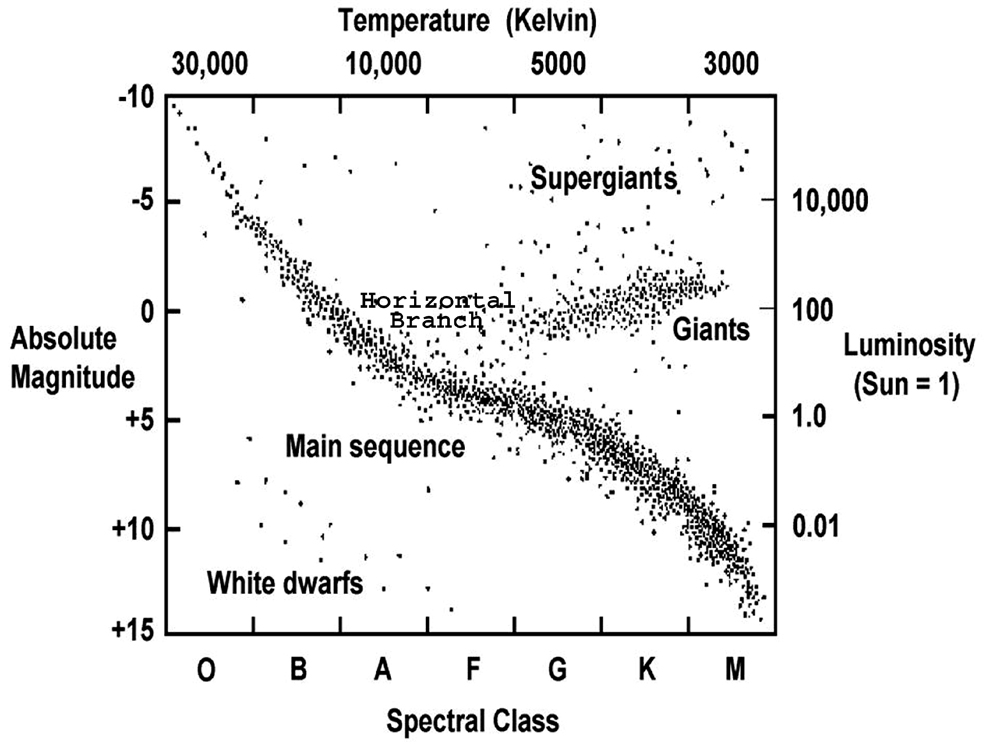
\includegraphics[scale=0.35]{gfx/Intro/HR_diagram} 
	\caption[Hertzsprung-Russell stars classification diagram.]{Hertzsprung-Russell stars classification diagram.}\label{fig:intro_HRdiagram}
\end{figure}

\section{The Learning Task}

We humans, like many other beings, are capable of learning a multitude of concepts throughout our lives, although generally the learning process is extremely slow. It takes us about six years to be able to begin dedicated and specific learning in primary education, and another eighteen years---generally speaking---to become computer scientists or experts in any other branch of knowledge.

Thus, the human learning process is a slow and tedious process. So, do we want to teach machines to learn the way humans do? Machines have proven to be outstanding at repetitive tasks, as well as they reach calculation speeds that humans can only dream of. It is worth asking if it is possible to develop a learning method for machines that is orders of magnitude faster than the human and equal or more effective. Although there is a major impediment to the development of such a method: we do not know if it exists! The search for a method to avoid the disadvantages of the human learning process is what drives research in the science we know today as \textit{machine learning}. 

One of the major differences between human learning and machine learning, and we must admit that to this respect machines again lead us, is the way in which knowledge is transferred. In machines it is enough to copy and paste, that is to say, once a program performs correctly the task for which it has been designed in a computer, it performs it in all of them. Just copy and paste. In humans this is not the case, we cannot extract knowledge from one brain and insert it into another, we don't even know how it is encoded! We humans must use our inefficient input-output devices to transmit knowledge. The following quote, which well reflects the reality of automatic learning, is more than thirty years old, yet still valid:

\begin{quotation}{\slshape
		...we do have reason to search for machine learning programs that will avoid the inefficiencies of human learning, although we must be alert to the possibility that such programs cannot, in principle, be constructed. The difficulty may be intrinsic in the task; human learning, though slow, may be close to optimally efficient.}
	\begin{flushright}
		\textbf{Herbert A. Simon, Machine Learning: An Artificial Intelligence Approach, 1983} 
	\end{flushright}
\end{quotation}

\section{Machine Learning}

So far, references have been made to learning without formally defining it. The concept of learning is deeply anchored in human beings. However, when trying to apply learning to computers, which are still no more than glorified calculators, we must give some kind of definition: \textit{Learning denotes changes in the system that are adaptive in the sense that they enable the system to do the same task or tasks drawn from the same population more efficiently and more effectively the next time} \cite{Michalski:2013:MLA:2588013}.

Machine learning is a field derived from computer science, and a branch of \acf{AI}, whose ultimate goal is to develop methods that make it possible for machines to learn. In other words, the techniques embedded in machine learning aim to develop programs that guide computers to learn from a set of examples. Machine learning is part of \acs{AI} in the sense that \acs{AI} is often directed at simulating human beings behavior through computers, so that we can better understand how humans work and help them.

\subsection{Types of Machine Learning} \label{sec:TypesOfML}

There are several approaches within the field of machine learning, these are classified according to the information that is provided to the machine for it to learn. Thus, following the classification proposed in \cite{ayodele2010types}, we find four different types of learning:

\begin{itemize}
	
	\item \textbf{Supervised Learning}: complete information is provided for learning. The machine is provided with a set of examples and the class (label) associated with each of them. The goal is to generate a function that approximates the behavior of the function that maps the examples in their respective classes.
	
	\item \textbf{Unsupervised Learning}: in this case the class to which the examples belong to is not available. The goal is to extract the class from the information contained in the set of examples.
	
	\item \textbf{Semi-supervised Learning}: it arises from adding incomplete information to unsupervised learning. This information is usually given in the form of a subset of labeled data, but there is no restrictions to this concern.
	
	\item \textbf{Reinforcement Learning}: the algorithm learns how to act under the influence of its environment, which provides feedback on the actions taken by the algorithm.
	
\end{itemize}

Among the four main categories of machine learning methods we find the \acf{SSL}, which is the focus of this work. As we have already mentioned, it is a machine learning paradigm that arises from adding incomplete information to unsupervised learning. We can divide \acs{SSL} methods into two broad categories according to their objective: semi-supervised classification and semi-supervised clustering \cite{chapelle2009semi}. The first method has partial information about the labels, so it tries to minimize the error based on them while taking into account the distribution of unlabeled instances. The second tries to obtain better defined clusters incorporating background information to the clustering process, this is known as constrained clustering and is the main subject of the study presented in this work \cite{triguero2015self}.

\section{Objectives}

The main objective of this work is to provide an overview of the concepts and particularities related to constrained clustering. Some of these concepts must be addressed with sufficient depth, in order for the reader to be able to easily understand the new approaches to constrained clustering contained in this work. It is also of our interest to provide an example of proper experimental methodology to obtain relevant and objectivity-free conclusions.

\section{Structure}

Regarding the organization of this work, background knowledge concerning classic clustering and constrained clustering will be presented in Chapters \ref{ch:IntroClustering} and \ref{ch:ConstrainedClustering} respectively. In Chapter \ref{ch:NewProposals} two new approaches to the constrained clustering problem are discussed. The experimental setup to carry out the experiments to test them and their results are presented in Chapters \ref{ch:ExperimentalSetup} and \ref{ch:ExperimentalResults} respectively. Afterward an empirical analysis of these results is performed in Chapter \ref{ch:AnalysisResults}. Finally conclusions and future work are discussed in Chapter \ref{ch:ConclFW}.

































	\part{Background}\label{pt:background}
	\chapter{Short Introduction to Clustering}\label{ch:IntroClustering}

Firstly, it will be necessary to provide an introduction, albeit a brief one, to clustering and its applications, in order to ease the understanding of the following chapters. For this purpose we will follow the study carried out in \cite{Everitt:2009:CA:1538772}. In Section  \ref{sec:ReasonsClassif} we present the reasons that lead humans to develop automatic classification methods. The numerical formulation for the latter is given in Section \ref{sec:NumMethClassif}. We give an intuitive definition for ``cluster'' in Section \ref{sec:WhatIsCluster}. Lastly a list of clustering application is presented in Section \ref{sec:ClusteringApplications}.

\section{Reasons for Classifying} \label{sec:ReasonsClassif}

Classification can be understood as a way of simplifying the information contained in large datasets in a way that is easily understood by humans. In this way, the processes of extracting useful information and applying it are simplified. Thus, if we are able to meaningfully divide a large dataset into subsets or groups, we can extract information common to elements of one of these subsets and provide a precise description that encompasses them.

The need to analyze information in this way grows with the emergence and availability of large datasets in science. The analysis of this type of information by classification, or clustering, is known today as \textit{Data Science}. In the 21st century a particular interest in data science arises from the appearance of the \textit{World Wide Web}, known as the Internet, where the aim has become to extract relevant information from the Web pages that make up this vast network.

It is important to note that, in most cases, there is no single classification criterion for the same dataset, but rather a wide variety of data. In the case of individuals, they could be classified, for example, on the basis of their income, or according to the amount of calories they consume over a defined period of time. Thus, different classification criteria do not necessarily result in the same division into groups of the set to be classified; in that way, different criteria will serve different purposes.

\section{Numerical Methods of Classification} \label{sec:NumMethClassif}

Numerical methods for clustering arise in branches of natural sciences, such as biology or zoology, in an attempt to eliminate the subjectivity implicit in the classification process triggered by the discovery of a new species. The aim is to provide a non-subjective and stable method for classifying and grouping elements.

These methods adopt different names that depend on the field in which they are applied: numerical taxonomy in biology, $Q$ analysis in psychology, or unsupervised pattern recognition in \acf{AI}. However, today, cluster analysis, or just clustering, are the most widely accepted and extended terms for tasks that involve the discovery of subgroups within a set of elements.

In most clustering applications, the goal is to obtain a data partition, in which each instance or object belongs to a single cluster, and the union of all of them contains all the individual objects. That said, it should be noted that, in some circumstances, solutions where there is overlap between clusters are acceptable, as well as there may not be an acceptable data partition.

In the literature, clustering methods are often divided into two subsets: partitional clustering and hierarchical clustering. In hierarchical clustering the result is not a partition of the data with a certain number of clusters---as in partitional clustering---, but instead a dendrogram in which there are partitions that include from the whole dataset to particular individuals \cite{Everitt:2009:CA:1538772}. A representative example of partitional clustering is the widely studied and well-known algorithm K-means \cite{wu2009top}, while for hierarchical clustering the CURE method should be highlighted \cite{guha1998cure}. In this work we will focus on partitional clustering.

The most common way to represent the information on which clustering is applied is an array $X$ of dimension $n\times u$, in which each row corresponds to an instance or object to be processed, and each column corresponds to one of the variables that characterize those instances or objects. The commonly accepted term to refer to each row is \textit{features vector}, and the features vector set is referred as \textit{dataset}.


$$ X = \left( \begin{array}{cccc}

x_{1,1} & x_{1,2} & \cdots & x_{1,u} \\

x_{2,1} & \cdots & \cdots & \cdots  \\

\vdots & \vdots & \vdots & \vdots \\

x_{n,1} & \cdots & \cdots & x_{n,u} \\

\end{array} \right) $$

The entry $x_{i,j}$ in $X$ corresponds to the value of the variable $j$th in the instance $i$. We will refer to the $i$th instance in $X$ as $x_i = (x_{[i,1]}, \cdots, x_{[i,u]})$, which is a feature vector.

We can define partitional clustering as the task of grouping the instances of the dataset $X$ into $k$ clusters, so that new information can be extracted from them. A typical clustering algorithm assigns a class label $l_i$ to each instance $x_i \in X$. As a result, we obtain the set of labels $L = \{l_1, \cdots, l_n\}$, with $l_i \in \{1, \cdots, k\}$, that effectively splits $X$ into $k$ non-overlapping clusters $\{c_i, \cdots, c_k\}$ to form a partition called $C$. The criterion used to assign an instance to a given cluster is the similarity to the rest of elements in that cluster, and the dissimilarity to the rest of instances of the dataset, which can be obtained with some kind of distance measurement $d(\cdot,\cdot)$ \cite{jain1999data}.

Variables in $X$ can be a mixture of attributes in a continuous, discrete, or categorical domain. In addition, it is possible that, in real problems, some entries may not be available. This mix of variable types and missing values can complicate the clustering task. However, there are methods to deal with these cases, such as inference of missing values or domain transformations.

In some applications, matrix rows may contain repeated measurements of the same variable, although under different conditions, or at different times, even at different spatial locations. An example of this can be the height measurements of a group of children in the same month over different years. This type of data has a structure that, again, can complicate the task of clustering.

Some clustering methods involve making transformations on the $X$ matrix to convert it into a $n \times n$ matrix in which measurements extracted from the $X$ matrix are stored that relate one instance to all the others, such as similarity, distance or dissimilarity.

Clustering is, put simply, the discovery of groups in data, and should never be confused with methods of discrimination or assignment, known in \acs{AI} as Supervised Learning, as we have already mentioned in Section \ref{sec:TypesOfML}. 

Once the general structure of clustering methods has been defined, it would be justified to ask, what is a cluster? Section \ref{sec:WhatIsCluster} will try to answer this question.

\section{What is a Cluster?} \label{sec:WhatIsCluster}

So far, the terms cluster, group and class have been used in a completely intuitive way, with no need for any formal definition, a further proof of the innate nature of these concepts in the human being. In fact, giving a formal definition of cluster is a task, not only complicated, but in many occasions not very useful. For example, in \cite{lance1967general} a cluster definition completely dependent on the user's interpretation is proposed. As far as this definition is concerned, a cluster is what the user understands as a cluster without having proposed a formal definition of it.

\begin{quotation}{\slshape
		The value judgment of the user is the ultimate criterion for evaluating the meaning of these terms [cluster]. If using them produces an answer of value, no more need be asked of them.}
	\begin{flushright}
		\textbf{R.E. Bonner, On Some Clustering Techniques, 1964} 
	\end{flushright}
\end{quotation}

Although the definition above is accurate in a wide range of situations, a somewhat more analytical definition from the mathematical point of view, defining a cluster in terms of internal cohesion---homogeneity---, and external isolation---separation is proposed in \cite{cormack1971review} and \cite{gordon:1999}. Figure \ref{fig:ClustersProperties} informally illustrates the properties described above, so that any observer will find the clusters present in it apparent without the need for a formal cluster definition. This may explain why achieving a mathematically accurate definition of homogeneity and separation may become unnecessary.

\begin{figure}[bth]
	\myfloatalign
	{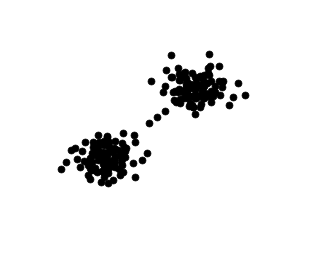
\includegraphics[width=.3\linewidth]{gfx/Clustering/TwoBasicsClusters}}
	{
\includegraphics[width=.3\linewidth]{gfx/Clustering/MoonsBasics}}
	{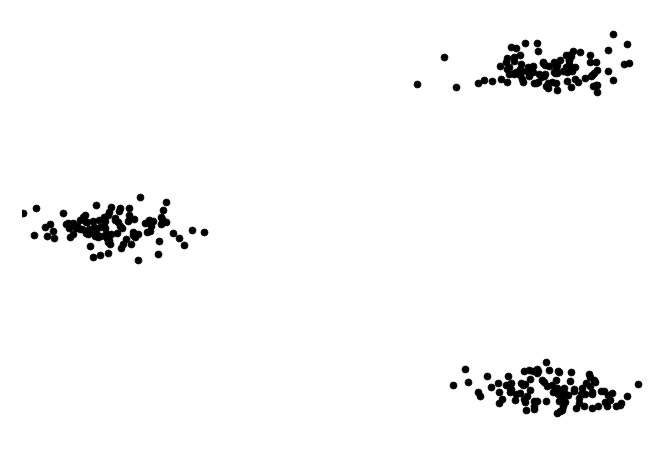
\includegraphics[width=.3\linewidth]{gfx/Clustering/ThreeBasicClusters}}
	\caption[Clusters with internal cohesion and/or external isolation]{Clusters with internal cohesion and/or external isolation}\label{fig:ClustersProperties}
\end{figure}

It is not entirely clear how people recognize different clusters when they are represented on a plane, but one of the variables that certainly influences is the distribution of relative distances between objects or points.

On the other hand, as mentioned earlier in this section, it may be the case that there is no justified partition in a dataset. Figure \ref{fig:uniform_cloud} shows a dataset for which most observers would conclude that there are no distinct groups, just a cloud of uniformly distributed points. Ideally, one would expect a clustering method applied to this same dataset to reach the same conclusion.

\begin{figure}[!h]
	\centering
	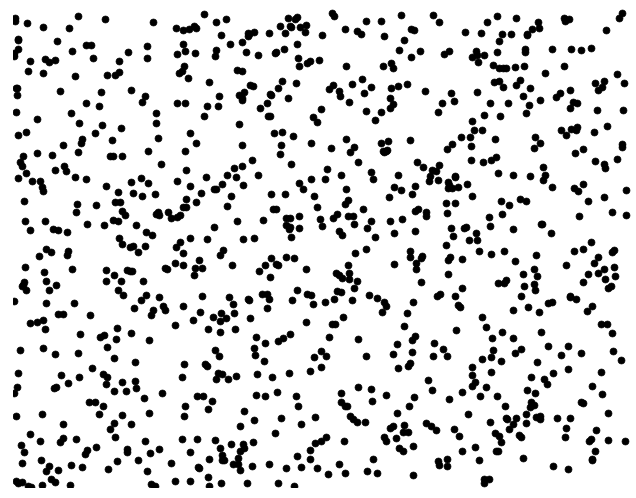
\includegraphics[scale=0.2]{gfx/Clustering/rand.png} 
	\caption{Cloud of uniformly distributed points.}\label{fig:uniform_cloud}
\end{figure}

However, most unsupervised learning methods will result in uniform partitioning as shown in Figure \ref{fig:uniform_partition}. The number of partitions found will depend on the method applied, although uniform partitioning will be achieved in any case.

\begin{figure}[!h]
	\centering
	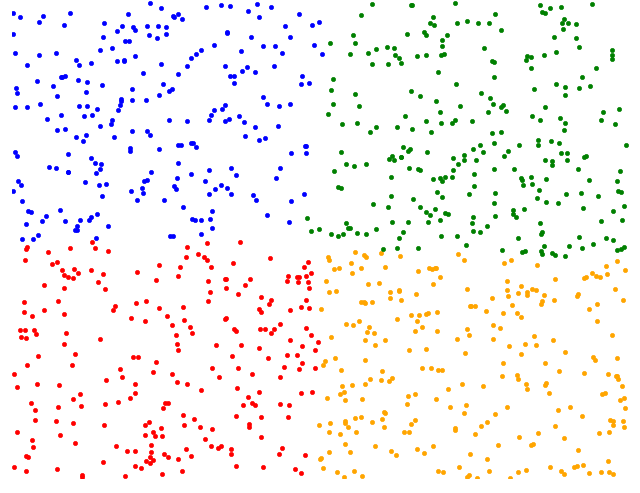
\includegraphics[scale=0.2]{gfx/Clustering/randClasif.png} 
	\caption{Classified cloud of uniformly distributed points.}\label{fig:uniform_partition}
\end{figure}

The process of dividing a homogeneous distribution of data into different groups is known as dissection, and such a process may be useful in certain circumstances. However, since in most cases of actual application of cluster methods, the structure of the data is not known a priori, there is risk of interpreting all solutions in terms of the existence of subgroups, which would lead to the imposition of a fictitious structure on data in which there is no structure present.

\section{Applications of Clustering} \label{sec:ClusteringApplications}

As it has been already mentioned, the general problem clustering attempts to solve is present in many disciplines: biology, botany, medicine, psychology, geography, marketing, image processing, psychiatry, archaeology, etc. This section presents some of the clustering applications related to these and others knowledge fields.

\subsection{Marketing}

Dividing customers into homogeneous groups is one of the most common marketing tasks. A marketing manager might wonder how to group potential customers according to the potential benefits of the product he or she is trying to introduce to the market. On the other hand, a marketing analyst might be interested in grouping companies according to their financial characteristics, in order to be able to analyze them and predict their market strategies.

An example of the application of clustering in this field was published in \cite{green1967cluster}. With a large number of cities available for analysis, they had to restrict the places in which to carry out their studies for economic reasons. To this end they relied on cluster analysis, classifying cities into small groups based on 14 city features, including size and average income \textit{per capita}. Since cities in the same group were expected to be very similar, they chose one city from each of them to conduct their studies.

Another application of cluster analysis in marketing was described in \cite{chakrapani2004statistics}. In this case, a car manufacturer believes that buying a sports car is not a decision based solely on economic capabilities or age, but is a lifestyle decision made by those who decide to buy a sports car, as opposed to those who do not. Consequently, the manufacturer decides to carry out a study, using cluster analysis, which allows it to identify all features related to the people who would buy a sports car, in order to focus its marketing campaigns specifically on this sector.

\subsection{Astronomy}

Given a set of astronomical data, researchers want to know, for example, how many classes of stars are present in them, based on some statistical criteria. The most frequently asked questions in this area are: how many statistically different objects are present in the data and to which class should each object be assigned? Do previously unknown classes of objects appear? Cluster analysis can be applied to answer these questions, helping to detect statistically anomalous objects, as well as to guide the process of classifying them. Examples include the discovery of high redshift quasars, type 2 quasars (highly luminous, active galactic nuclei often obscured by dust and gas), and brown dwarfs.

In \cite{faundez1996classification} a specific example of the above can be found. Clustering techniques are applied to data on the chemical composition of 192 planetary nebulae. Six different groups were identified, which were similar in many respects to a previous classification of such objects, but also showed interesting differences that researchers had so far missed.

Clustering based on normal distributions is applied to a set of 2370 stars in \cite{celeux1992classification}. They were described by their relative speed to the galactic nucleus and galactic rotation. Using a model of three clusters, they found one cluster of large size and small volume, and two of small size and large volume.

\subsection{Psychiatry}

Mind disorders are often more difficult to diagnose than body pathologies, which is why there has been a growing interest in cluster analysis techniques to refine, or even redefine, diagnostic techniques for this type of disease in the field of psychiatry. Much of this work involves depressed patients, cases in which the interest lies in distinguishing between two types of depression, endogenous (congenital) and neurotic.

In \cite{pledger2008using} clustering techniques are applied to 200 patients based on their responses to a questionnaire about depression, along with information about their sex, age, mental state, and illness. This is a clear example of different types of variables included in the same dataset. One of the groups obtained as a result of this study was identified as a marker of endogenous depression.

Cluster analysis has also been used to find a classification of individuals who attempted suicide, which could lay the groundwork for further studies on the causes and treatments of the problem. In \cite{paykel1978classification} a study on 236 cases of failed suicides recorded by the emergency service of a city in the United States of America is presented. From the set of available variables, 14 were selected as particularly relevant for classification and, therefore, were used in the analysis. Among them were: age, number of suicide attempts, severity of depression and degree of hostility, in addition to a series of demographic features. Clustering methods were applied to the resulting dataset; the most significant result obtained corresponds to a division into three well-defined clusters.

\subsection{Meteorology and Climatology}

Huge amounts of global weather data are collected daily. Exploring these data using clustering techniques can bring new approaches to study climatology and environmental phenomena.

In \cite{littmann2000empirical} clustering techniques are applied to data collected on daily changes in surface pressure in the Mediterranean basin, 20 groups explaining the variance of rainfall in the central Mediterranean regions were found. Another example can be found in \cite{liu2005mining}, in which the Fuzzy K-means algorithm is applied to spatial-temporal data of the USA southern-central regions climatology. 

\subsection{Archaeology}

Archaeology is another discipline in which clustering is useful. The classification of different objects found in deposits can help to discover their use, the periods to which they belong, as well as the population that used them. Similarly, studying fossilized materials can help reveal how prehistoric societies lived. 

An early example of the application of clustering to archaeological objects is given in \cite{hodson1966some}, where clustering techniques are applied to a group of brooches dating from the Iron Age, finding a classification for them of proven archaeological relevance. Another example found in \cite{hodson1971numerical} is the application of the K-means algorithm to construct a taxonomy of hand axes found in the British Isles. The variables taken into account to describe each axe include length, width and pointedness. Clustering resulted in two groups of axes, one made up of small and thin axes and the other made up of large and thick axes.

Regarding fossilized materials, in \cite{sutton1995cluster} a study of 155 coprolites found at Antelope House, a prehistoric site at Chelly Canyon in Arizona is conducted. The study resulted in a diet-based interpretation of the differences between coprolites.

\subsection{Bioinformatics and Genetics}

Recent times are witnessing a tremendous boom in interest in Bioinformatics, complemented by molecular biology, computer science, mathematics and statistics. Such an increase has been accelerated by the ever-growing database of genomic and protein data, which are themselves the result of a major advance in DNA sequencing techniques, gene expression measurements, and compression of macromolecular structures. Statistics have been relevant in the study of gene expression. The genes contained in the DNA of each cell provide the necessary templates for the generation of the proteins involved in most of the structural and biomechanical processes that take place in each of us. However, although most cells in humans contain all the genetic components that make up the human genome, genes are expressed selectively in each cell depending on cell type, tissue and general conditions inside and outside the cell. Molecular biology has shown that most of the processes in a cell's life are regulated by factors that affect the expression of its genes.

As we have seen, one of the most active fields of research today is the study of the processes that regulate gene expression. In order to store the information related to this area of study, microarrays arise \cite{cortese2000array}. From the data analysis point of view, one of the relevant features in this type of information is that the number of attributes of each instance ($u$) far exceeds the number of available instances ($n$); datasets featuring this property are called \textit{high dimensionality datasets}.

Most classic statistical methods cannot be applied to this type of dataset without being substantially modified. However, cluster analysis accepts such datasets and can be used to identify groups of genes with similar expression patterns. This allows us to answer questions such as why a gene is affected by a certain disease, or which genes are responsible for hereditary genetic diseases.

An example of application is found in \cite{selinski2008cluster}, who used clustering on single-nucleotide polymorphisms to detect differences between diseases at the genetic level.

\section{Recent Applications}

Although the examples of practical clustering applications presented so far are illustrative, it should be noted that clustering techniques are applied in a multitude of modern problems. Since it is not humanly possible to cover all the practical uses of clustering, a brief list of some of them is presented here: computer vision-guided traffic management \cite{kumaran2019computer}, near real-time detection of
spatial clusters from large position data streams generated
by moving objects \cite{junior2019dg2cep}, wireless sensor networks management \cite{wan2019similarity}, internet of things \cite{aranzazu2019anchor}, detecting taxi movements \cite{ibrahim2019detecting}, \textit{big data} distributed multi-target regression \cite{corizzo2019dencast},  cartographic labeling \cite{araujo2019improving} and image segmentation in various fields, ranging from general applications \cite{wang2018non} to very specific ones such as in medicine \cite{verma2016improved, aparajeeta2016modified}. 

It seems clear that clustering is an extremely powerful tool, no only for the development of any branch of science, but also because it can be applied to  many real-world problems and directly help people.

\section{Summary}

Clustering consists of exploring datasets. Its goal is to determine whether or not they can be summarized in a meaningful way, in terms of a relatively small number of groups or clusters of objects or individuals which resemble each other and differ from those found in other clusters.

Many branches of science have successfully made use of clustering techniques to advance in their respective fields and to process large amounts of data, whose analysis would be unthinkable to tackle with traditional techniques.

%Para referir un acronimo completo \acf
%Para referir un acronimo solo con las siglas \acs





















	\chapter{Constrained Clustering}\label{ch:ConstrainedClustering}

Once the basics concepts about clustering have been introduced, we can focus on defining the concepts specific to constrained clustering. We give example applications and highlight its advantages and disadvantages. To this end we take as our main reference the survey presented in \cite{davidson2007survey}. We describe the motivation for constrained clustering in Section \ref{sec:CCMotiv}. We formalize the concept of constraints and discuss their use in Sections \ref{sec:ConstDef} and \ref{sec:ConstUse} respectively. Afterwards a list of applications of constrained clustering is presented in Section \ref{sec:CCApplications}. Benefits and problems, as well as solutions for these problems, are discussed in Sections \ref{sec:ConstraintsBenefits} and \ref{sec:ConstraintsProblems} respectively.

\section{Motivation for Constrained Clustering} \label{sec:CCMotiv}

As we discussed in Chapter \ref{ch:IntroClustering}, unsupervised clustering methods are useful for structuring data referring to a particular area. An example of this can be found in text classification; In \cite{cohn2003semi} a problem proposed by Yahoo! is addressed. The problem consists in, given a large number of text documents, grouping them according to a taxonomy in which documents with similar topics are conceptually nearby. To solve this problem, unsupervised clustering methods are useful, as there is limited initially available information on the problem. However, in \cite{wagstaff2001constrained} it is shown that applying unsupervised clustering to certain problems, such as grouping \acf{GPS} data in such a way that clusters define the lanes of a road, does not produce significant results, as the clusters obtained are far from the elongated shape that would be expected. To tackle the problem, they introduced a new element in clustering, the \textit{constraint}, which made it possible to include domain knowledge to guide clustering methods towards the expected results. It was enough to indicate that the lanes of the road on which the vehicles circulate are four meters wide, and therefore any vehicle that is at a distance of more than 4 meters from another, perpendicular to the motion direction, must be located in a different cluster.

We are now in a new scenario: it is possible to incorporate additional information into the clustering process, in addition to that contained in the dataset itself, to guide it in the formation of the output partition and obtain more accurate results. This new approach is known as constrained clustering, an \acf{SSL} paradigm, unlike traditional clustering methods which fall into the category of unsupervised learning. 

\section{Constraints Definition} \label{sec:ConstDef}

The new type of information that we incorporate into clustering is given in the form of instance-level constraints. Their purpose is to specify whether two instances ($x_i$ and $x_j$) from the dataset ($X$) must be in the same cluster or, on the contrary, they must be in separate clusters.

Constraints that indicate that two instances must be placed in the same cluster are called \acf{ML}, and are noted with $C_=(x_i,x_j)$. Similarly, constraints that specify that two instances must not be placed in the same cluster are called \acf{CL}, and are noted with $C_{\neq}(x_i,x_j)$ \cite{wagstaff2000clustering}.

Although they may seem simple, constraints defined as above have some very interesting properties. \acs{ML} constraints are an example of an equivalence relation, and therefore are symmetrical, reflexive and transitive. Observation \ref{ob:MLConstraintsRelation} formalizes this concept. On the other hand, and although \acs{CL} do not constitute an equivalence relation, they feature other properties, formalized in Observation \ref{ob:CLConstraintsRelation}.

\begin{observation}
	\textbf{Must-link constraints are transitive.} Let $CC_i$ and $CC_j$ be connected components (completely connected subgraphs by \acs{ML} constraints), and let $x_i$ and $x_j$ be the instances in $CC_i$ and $CC_j$ respectively. Then $C_=(x_i,x_j): x_i \in CC_i, x_j \in CC_j \rightarrow C_=(x_a,x_b) \forall x_a, x_b: x_a\in CC_i, x_b \in CC_j$ \cite{davidson2007survey}.
	\label{ob:MLConstraintsRelation}
\end{observation}

\begin{observation}
	\textbf{Cannot-link constraints can be entailed.} Let $CC_i$ and $CC_j$ be connected components (completely connected subgraphs by \acs{CL} constraints) and let $x_i$ and $x_j$ be the instances in $CC_i$ and $CC_j$ respectively. Then $C_{\neq}(x_i, x_j): x_i \in CC_i, x_j \in CC_j \rightarrow _{\neq}(x_a, x_b) \forall x_a, x_b: x_a\in CC_i, x_b \in CC_j$ \cite{davidson2007survey}
	\label{ob:CLConstraintsRelation}.
\end{observation}

A clear example of the use of constraints can be found in clustering applications where there are distance measurement limitations, as in the case of \acs{GPS} data. Thus, if we want instances forming two clusters to be separated by a distance greater or equal to $\delta$, it is enough to set \acs{ML} constraints between all instances separated by less than $\delta$ units. Similarly, if we want the diameter of the clusters to be at most $\epsilon$, we must set \acs{CL} constraint between instances separated by more than $\epsilon$ units. Figure \ref{fig:DistanceConstraints} shows a graphical representation of these two types of constraints.

\begin{figure}[!h]
	\centering
	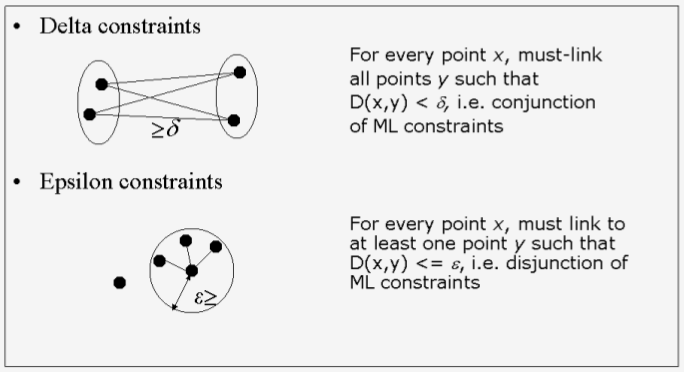
\includegraphics[scale=0.45]{gfx/ConstClust/RestriccionesDeltaEpsilon.png} 
	\caption[\textit{delta} $(\delta)$ and \textit{epsilon} $(\epsilon)$ constraints.]{\textit{delta} $(\delta)$ and \textit{epsilon} $(\epsilon)$ constraints \cite{davidson2007survey}.}\label{fig:DistanceConstraints}
\end{figure}


\section{Use of Constraints} \label{sec:ConstUse}

While supervised learning involves knowing the label associated with each instance, \acs{SSL} has only a subset of labeled instances. On the other hand, in many domains the available information refers to relations between instances, and not to the specific class to which they belong. Moreover, in interactive clustering systems, a user who is not expert in the problem domain will probably be able to provide information in the form of constraints such as \acs{ML} and \acs{CL}, instead of providing information on what particular class certain instances belong to \cite{cohn2003semi,davidson2007hierarchical}.

Typically, constraints are incorporated into clustering problems in two ways. They can be used to alter the rules of assignment of instances to clusters of the method in question, so that the solution satisfies as many constraints as possible. Alternatively, it is possible to train the distance function used by the method based on the constraints, either before or during the application of the method. In any case, the initialization phase can take the constraints into account, so that instances appearing together in \acs{ML} constraints will be placed in the same cluster, and those between which there is a \acs{CL} constraint will be placed in different clusters. Based on this distinction, we identify two ways of approaching the problem: those based on explicit constraints (\textit{constraints-based}) and those based on distances (\textit{distance-based}).

\subsection{Constraints-based Methods}

In constraints-based methods, the clustering method itself is modified in such a way that the available information is used to bias the search and obtain an appropriate data partition.

Regarding the degree to which the constraints have to be satisfied, we can make a distinction between the concepts of hard \cite{wagstaff2001constrained,davidson2005agglomerative} and soft \cite{law2004clustering,basu2004active,segal2003discovering,davidson2005clustering,law2005model} constraints. Hard constraints must necessarily be satisfied in the output partition of any algorithm that makes use of them, while soft constraints are taken as a strong guide for the algorithm that uses them but can be partially satisfied in the output partition \cite{seret2014new}. For the purposes of this work, we will employ the latter. There are several techniques to obtain a partition based on constraints:

\begin{itemize}
	
	\item Modifying the objective function to include a penalty term for breaking constraints \cite{demiriz1999semi,davidson2005clustering}.
	
	\item Grouping instances with additional information obtained from a conditional distribution into an auxiliary space \cite{sinkkonen2000semisupervised}.
	
	\item Enforcing all constraints to be satisfied by modifying the the instance clusters assignment rule \cite{wagstaff2001constrained}.
	
	\item Initializing clusters based on constraints inferred from a set of labeled instances \cite{basu2002semi}.
	
\end{itemize}

Figure \ref{fig:ConstClustOverDataset} shows a dataset together with its associated constraints and proposes a possible clustering that satisfies all constraints.

\begin{figure}[bth]
	\myfloatalign
	\subfloat[Constraints over a dataset.]
	{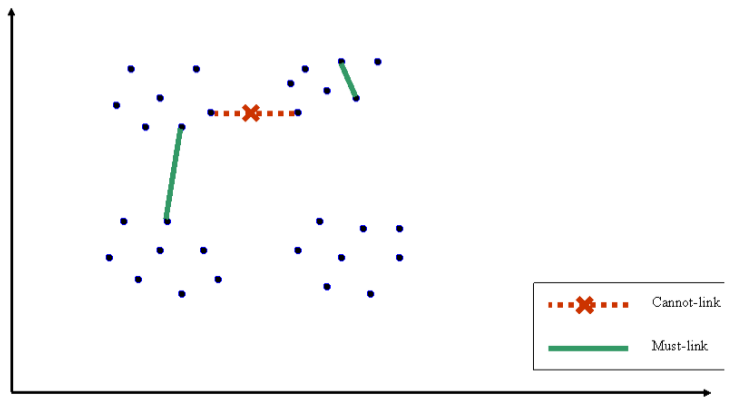
\includegraphics[width=.45\linewidth]{gfx/ConstClust/InputInstancesAndConst1}}
	\hspace{1cm}
	\subfloat[Clustering satisfying all constraints.]
	{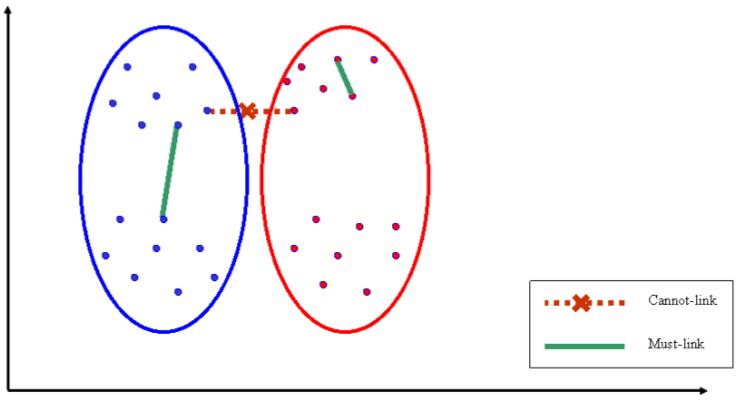
\includegraphics[width=.45\linewidth]{gfx/ConstClust/ClusteringSatAll}}
	
	\caption[Constraints and clustering over a dataset.]{Constraints and clustering over a dataset \cite{davidson2007survey}.} \label{fig:ConstClustOverDataset}
\end{figure}

\subsection{Distance-based Methods}

In distance-based approaches, classic clustering methods that use a distance measurement are modified so that the distance measurement incorporates the constraints. In this context, constraint satisfaction means that instances co-occurring in \acs{ML} constraints are placed together in the space, and those co-occurring in \acs{CL} are separated.

Figure \ref{fig:ConstrainsAndMetricLearned} shows a possible clustering based on a metric learned from the constraints. It should be noted that in Figure \ref{fig:MetricLearned} the data space has been compressed on the vertical axis and expanded on the horizontal axis to match the learned distance metric.

\begin{figure}[bth]
	\myfloatalign
	\subfloat[Constraints over a dataset.]
	{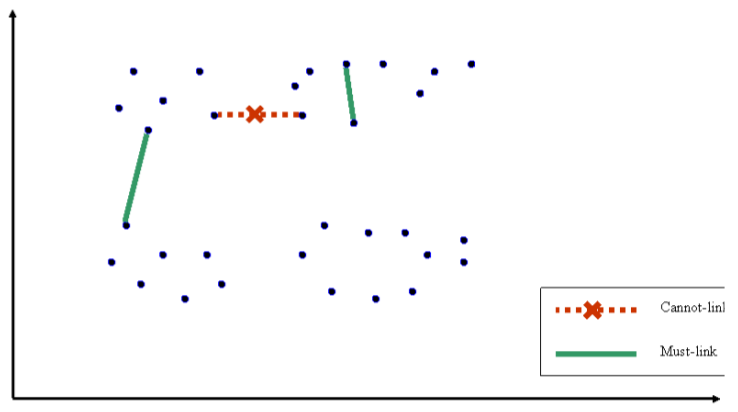
\includegraphics[width=.45\linewidth]{gfx/ConstClust/InputInstancesAndConst2}} 
	\hspace{0.5cm}
	\subfloat[Clustering based on a metric learned from constraints.]
	{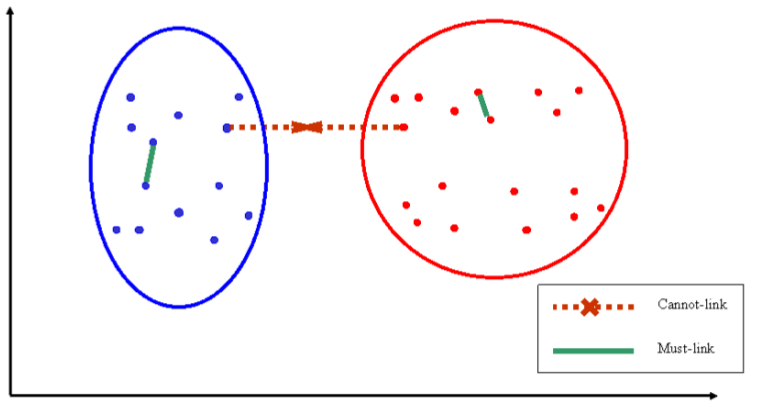
\includegraphics[width=.45\linewidth]{gfx/ConstClust/MetricaAprendida}
	\label{fig:MetricLearned}}
	\caption[Clustering based on a metric learned from constraints.]{Clustering based on a metric learned from constraints \cite{davidson2007survey}.} \label{fig:ConstrainsAndMetricLearned}
\end{figure}

\section{Constrained Clustering Applications} \label{sec:CCApplications}

This section shows some application cases in which constrained clustering has turned out to be a more useful tool than fully unsupervised clustering. For each case we will analyze how the constraints were obtained and how they improve the resulting clustering. 

\subsection{Image Analysis}

Figure \ref{fig:CMUFacesDatabase} shows a sample from the \acsfont{CMU} (Carnegie Mellon University) faces dataset, where the task is to group faces according to different criteria (in this case, face orientation).

\begin{figure}[bth]
	\myfloatalign
	\subfloat[Profile faces.]
	{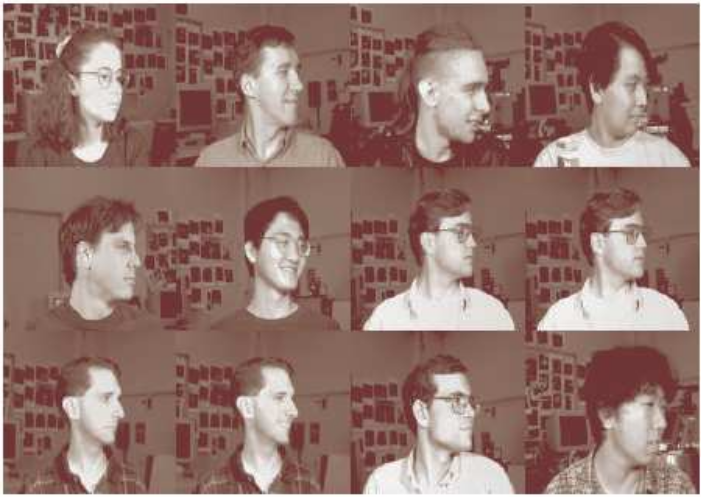
\includegraphics[width=.3\linewidth]{gfx/ConstClust/AnalisisImagenes/Caras1}} \quad
	\subfloat[Front faces.]
	{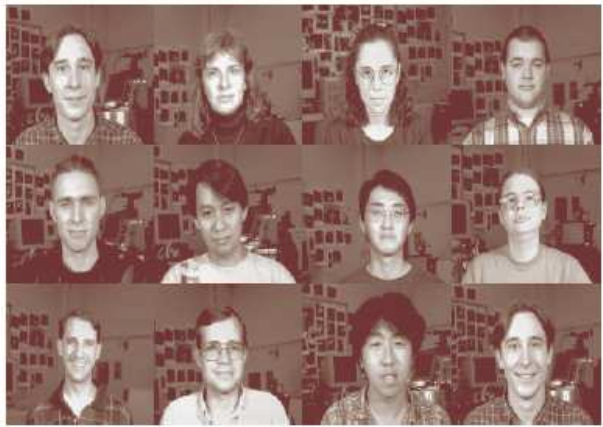
\includegraphics[width=.3\linewidth]{gfx/ConstClust/AnalisisImagenes/Caras3}} \quad
	\subfloat[Faces up.]
	{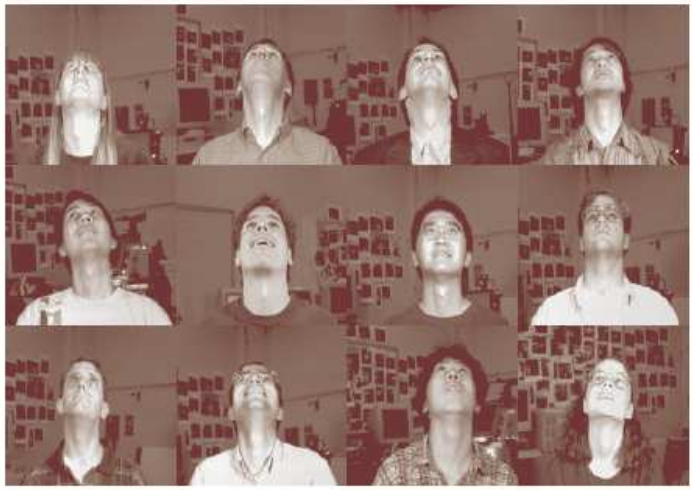
\includegraphics[width=.3\linewidth]{gfx/ConstClust/AnalisisImagenes/Caras2}} \quad
	\caption[\acsfont{CMU} faces database.]{\acsfont{CMU} faces database \cite{davidson2007survey}.}\label{fig:CMUFacesDatabase}
\end{figure}

The method used to obtain the constraints is one of the most popular in the literature: let the number of clusters of the resulting partition be equal to the number of classes in the database, and generate the constraints from a subset of labeled instances; in other words, if two instances have different labels, set a \acs{CL} constraint between them, and otherwise set an \acs{ML} one. Thus, between the images shown in Figure \ref{fig:FacesDatabaseCL} \acs{CL} constraints are set, since, although they depict the same person, they do not have the same orientation.

\begin{figure}[bth]
	\myfloatalign
	{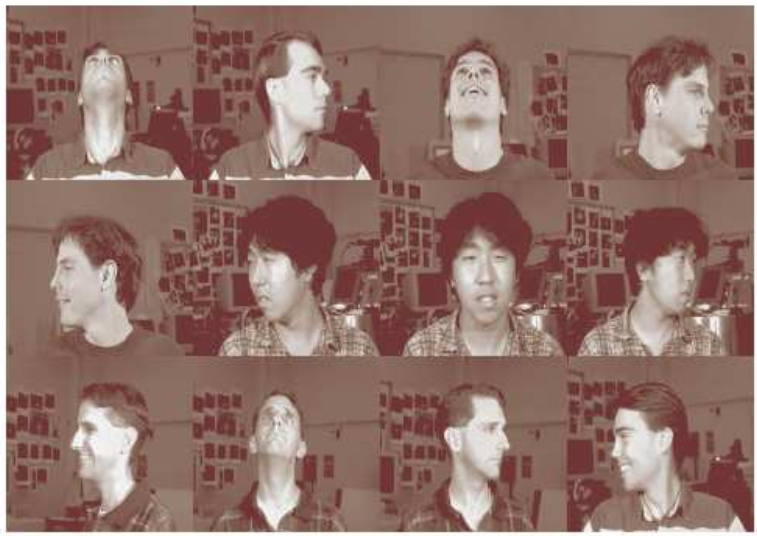
\includegraphics[width=.35\linewidth]{gfx/ConstClust/AnalisisImagenes/CarasDifOr1}} \quad
	{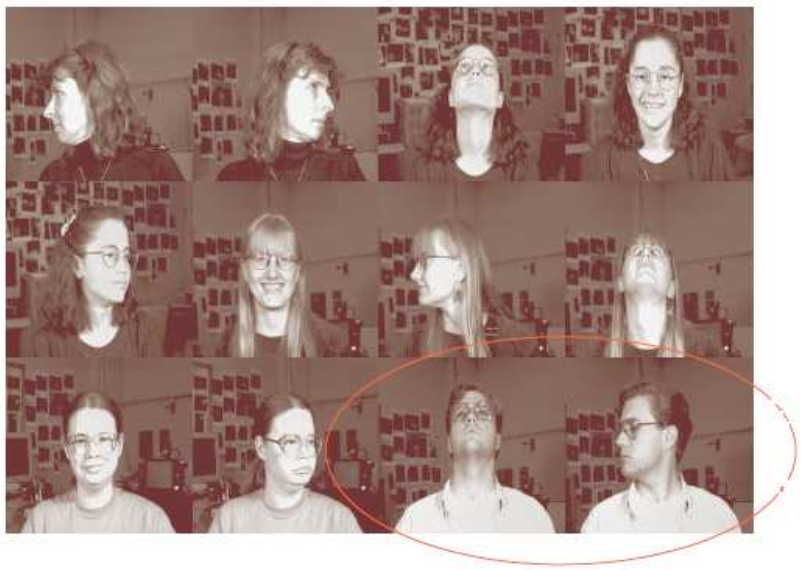
\includegraphics[width=.35\linewidth]{gfx/ConstClust/AnalisisImagenes/CarasDifOr2}}
	\caption[\acs{CL} constraints between faces of the same person.]{\acs{CL} constraints between faces of the same person \cite{davidson2007survey}.}\label{fig:FacesDatabaseCL}
\end{figure}

Figure \ref{fig:AiboRobotClustSys} shows another set of image data to which constrained clustering techniques are applied. In this case, the task is to perform object recognition to incorporate the method into the navigation system of the Aibo robot \cite{davidson2005clustering}. Distance constraints such as $\delta$ and $\epsilon$ are used as described in Figure \ref{fig:DistanceConstraints}. In this way, well differentiated clusters are obtained and therefore they are useful for the path-finding tasks performed by the robot during navigation.

\begin{figure}[bth]
	\myfloatalign
	\subfloat[Original image.]
	{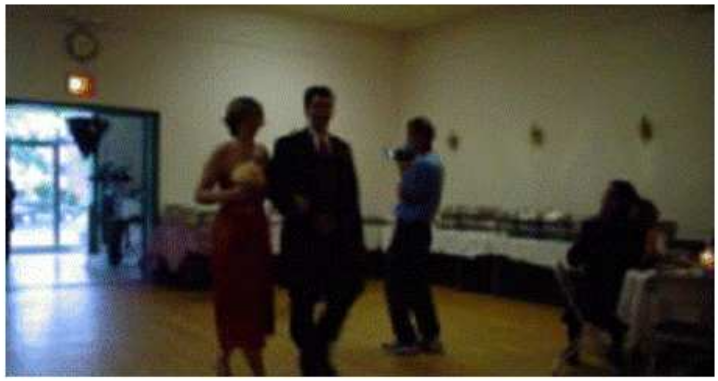
\includegraphics[width=.3\linewidth]{gfx/ConstClust/AnalisisImagenes/Aibo1}} \quad
	\subfloat[Classic clustering.]
	{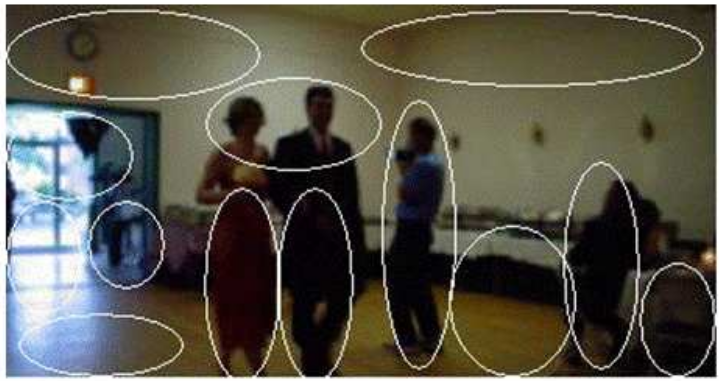
\includegraphics[width=.3\linewidth]{gfx/ConstClust/AnalisisImagenes/Aibo2}} \quad
	\subfloat[Constrained clustering.]
	{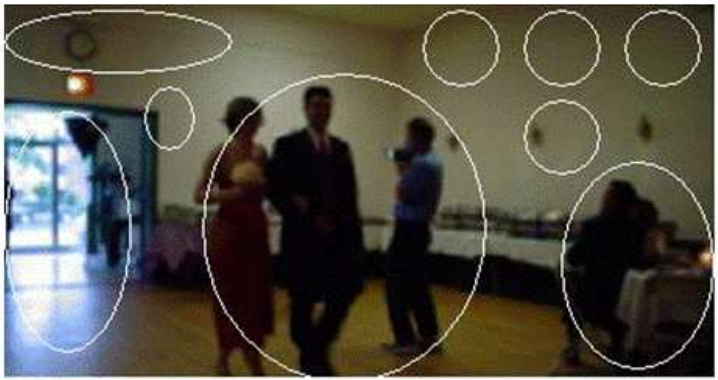
\includegraphics[width=.3\linewidth]{gfx/ConstClust/AnalisisImagenes/Aibo3}} \quad
	\caption[Clustering method used in Aibo robot navigation system.]{Clustering method used in Aibo robot navigation system \cite{davidson2007survey,davidson2005clustering}.}\label{fig:AiboRobotClustSys}
\end{figure}

\subsection{Video Analysis}

Video databases are one example where constraints can be generated directly from the data domain, especially if space-time metadata is available \cite{yan2006discriminative}. In time-sequenced data it is possible to set \acs{ML} constraints between groups of pixels of frames close in time. This is especially useful when the task is to perform object recognition based on clustering and segmentation. It is also possible to add \acs{CL} constraints to image segments in the same snapshot, as the probability of them being associated with the same object after segmentation is low. In fact, in video analysis problems there are a variety of constraint extraction methods \cite{yan2006discriminative}. Figure \ref{fig:ConstExtractionVideo} shows some examples. 

\begin{figure}[bth]
	\myfloatalign
	\subfloat[]
	{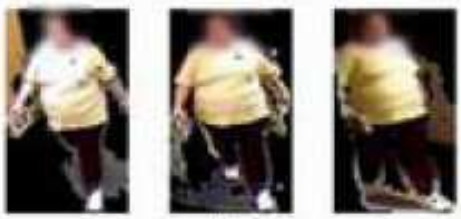
\includegraphics[width=.4\linewidth]{gfx/ConstClust/Videos/VideoA}
	\label{fig:ConstExtractionVideoA}}
	\quad
	\subfloat[]
	{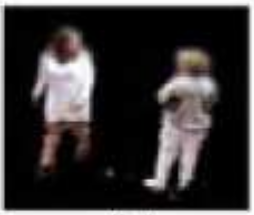
\includegraphics[width=.225\linewidth]{gfx/ConstClust/Videos/VideoB}
	\label{fig:ConstExtractionVideoB}} \quad
	\subfloat[]
	{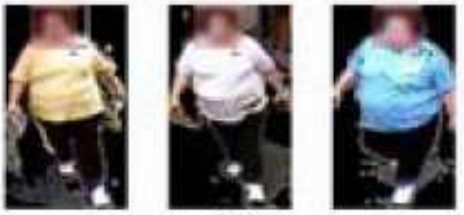
\includegraphics[width=.4\linewidth]{gfx/ConstClust/Videos/VideoC}
	\label{fig:ConstExtractionVideoC}}
	\quad
	\subfloat[]
	{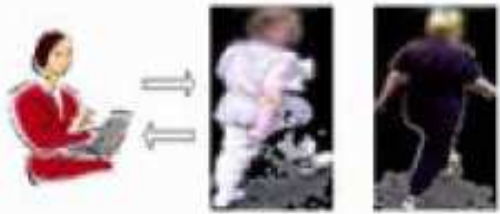
\includegraphics[width=.4\linewidth]{gfx/ConstClust/Videos/VideoD}
	\label{fig:ConstExtractionVideoD}}
	\caption[Constraints extraction in video data.]{Constraints extraction in video data \cite{yan2006discriminative,davidson2007survey}.}\label{fig:ConstExtractionVideo}
\end{figure}

In Figure \ref{fig:ConstExtractionVideo}, image \ref{fig:ConstExtractionVideoA} corresponds to constraints extracted from tracking a person over a period of time; \ref{fig:ConstExtractionVideoB} corresponds to spatial constraints associating two objects located in the same frame; image \ref{fig:ConstExtractionVideoC} corresponds to constraints obtained through facial recognition, and \ref{fig:ConstExtractionVideoD} to those provided by the user.

With so many constraint extraction methods, one might ask: What happens if too many constraints are imposed? Does this make the problem over-constrained? In Section \ref{sec:ConstraintsProblems} we will address these questions.

\subsection{Biological Data}

In gene clustering based on microarray data, genes are represented by their expression profile in different experiments and grouped using different constrained clustering methods. Figure \ref{fig:GeneticApp} shows an example: these are \acs{ML} constraints set between genes based on co-occurrence data stored in the protein interaction database, which contains information about which genes---and their associated proteins---are present in the same cell processes \cite{xenarios2001dip}. This information can be used to improve results provided by clustering methods. \cite{segal2003discovering}.

\begin{figure}[!h]
	\centering
	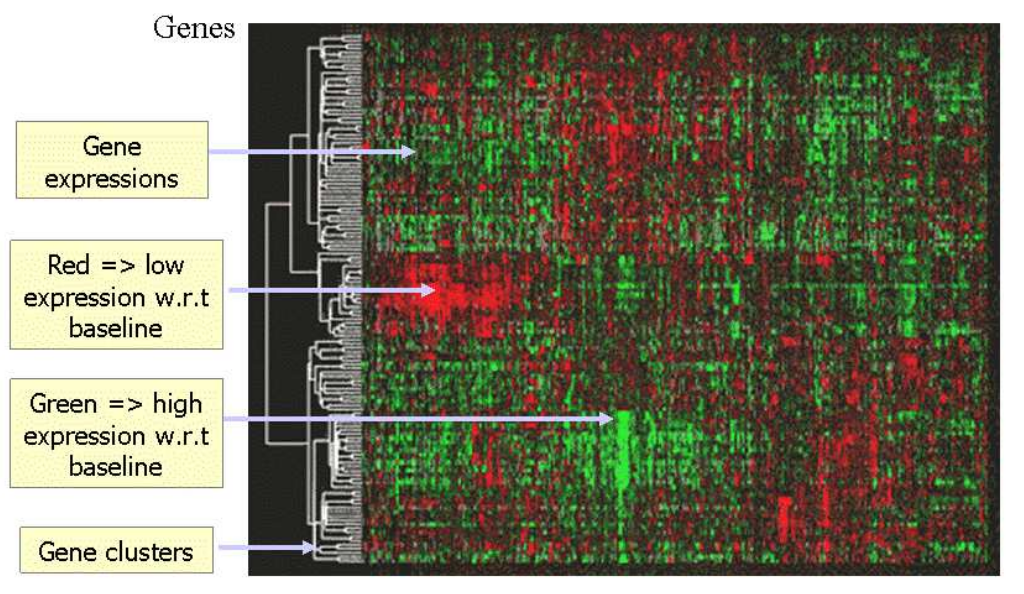
\includegraphics[scale=0.3]{gfx/ConstClust/Genetica/Genes} 
	\caption[Gene clustering based on microarray data.]{Gene clustering based on microarray data \cite{davidson2007survey}.}\label{fig:GeneticApp}
\end{figure}

\subsection{Text Analysis}

In content classification tasks, the goal is to automatically split large amounts of documents into groups or clusters. In this case it is possible to extract constraints from multiple auxiliary resources. For example, if two documents are in the same directory, an \acs{ML} constraint could be set between them. This way, it is possible to adjust the resulting clustering to suit a particular criterion, such as creating a hierarchy of documents akin to the way they are organized in the original directory structure.

\subsection{Web Data} 

Constrained clustering is very useful in web search data processing. Here, the aim is to automatically group the results of an ambiguous query to the search engine into clusters of \acsp{URL}, which represent the queried concept in different contexts. In this area it is possible to extract the constraints from previous searches performed by other users, so that an \acs{ML} constraint is set between \acsp{URL} visited in the same user session. Clustering using these constraints can help bias search results towards user preferences.

\subsection{Audio Data}

In certain audio analysis tasks, the number of object classes present in the data may not be known, although constraints can be extracted directly from the data domain. This happens, for example, when applying clustering to speaker recognition in a conversation \cite{bar2003learning}. In this case the number of participants is not known a priori, but it is easy to detect if two speakers are different or similar and to set constraints accordingly.

\subsection[\acsfont{GPS} Data]{GPS Data} \label{sec:GPSApp}

As mentioned at the beginning of Chapter \ref{ch:ConstrainedClustering}, constrained clustering can be applied to \acs{GPS} data in order to identify the lane each vehicle is in, as shown in Figure \ref{fig:GPSClustData}. Each instance is represented by the position it occupies on the road in two-dimensional Cartesian coordinates $(x,y)$ obtained from \acs{GPS} data. Figure \ref{fig:figure15} graphically shows this representation of the data. Note that multiple instances can refer to the same vehicle at different times.

\begin{figure}[!h]
	\centering
	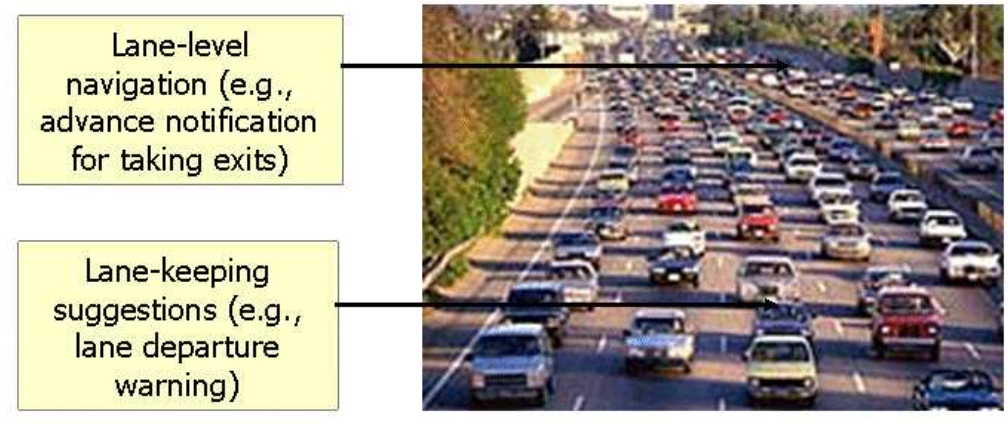
\includegraphics[scale=0.3]{gfx/ConstClust/GPS/Coches} 
	\caption[\acs{GPS} data use.]{\acs{GPS} data use \cite{davidson2007survey, wagstaff2001constrained}.}\label{fig:GPSClustData}
\end{figure}

In this domain, real clusters have an elongated shape on the horizontal axis and are aligned perpendicularly to the motion direction. To produce clusters with this shape, we can make use of constraints. We will set \acs{CL} constraints between those instances more than four meters apart perpendicularly to the motion direction---since the lanes have a maximum width of four meters---and \acs{ML} constraints between those instances that present continuity in the motion direction axis, since it is likely that the vehicles they represent are in the same lane. This clustering model has proven to be very useful in real-time navigation \cite{wagstaff2001constrained}, allowing for the user to be notified when to change lanes, or when not to.

\begin{figure}[!h]
	\centering
	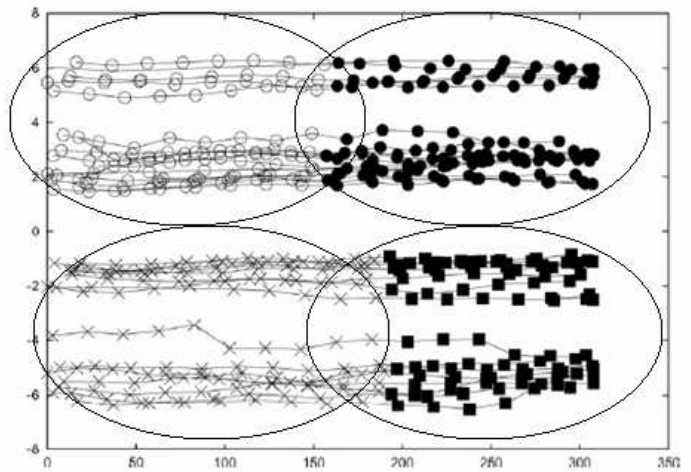
\includegraphics[scale=0.32]{gfx/ConstClust/GPS/Instancias} 
	\caption[Clustering of \acs{GPS} data with no constraints.]{Clustering of \acs{GPS} data with no constraints \cite{davidson2007survey,wagstaff2001constrained}.}\label{fig:figure15}
\end{figure}

\subsection{Recent Applications}

The aforementioned applications are the most studied in the literature, although the reader may have the impression that constrained clustering is no longer used in real-world problems. To prevent that, we provide a list of more recent applications of constrained clustering to modern problems: advanced robotics navigation systems \cite{semnani2016constrained}, applied marketing \cite{seret2014new}, obstructive sleep apnea analysis \cite{mai2018evolutionary}, handwritten digits classification \cite{li2015scalable}, Internet traffic classification \cite{wang2014internet}, electoral district designing, \cite{brieden2017constrained}, semantically similar relations identification \cite{wang2015constrained}, cooperative team building \cite{yang2014team}, video face clustering \cite{zhou2014video}, image clustering \cite{habashi2017semi} and storage location assignment in warehouses \cite{yang2016constrained}, among others.

\section{Benefits of Using Constraints} \label{sec:ConstraintsBenefits}

Two main benefits are found in the use of constraints:

\begin{itemize}
	
	\item Increased accuracy in label prediction by generating constraints based on a subset of labeled instances.
	
	\item Obtention of clusters with adaptable geometry to each problem.
	
\end{itemize}

These two benefits are discussed below:

Given $X = \{x_1 \cdots x_n\}$, a large set of unlabeled instances, and $L = \{(x_{n+1}, l_{n+1}) \cdots (x_{n+|L|}, l_{n+|L|})\}$, a small set of labeled instances, it is common to choose two elements from $L$ (with replacement) and set an \acs{ML} constraint between them if they belong to the same class, or a \acs{CL} constraint otherwise. An appropriate way to evaluate the results provided by a clustering method is to measure the level of accuracy it achieves when predicting dataset $X$ labels. This normally requires the number of desired clusters to be equal to the number of known classes in $X$ ($k = k^*$). Methods such as the RandIndex \cite{rand1971objective} or its variants, which will be discussed later, are used to measure the degree of agreement between two given partitions (clusterings).

In \cite{wagstaff2000clustering}, where constraints are generated as described above, it is shown that accuracy is increased up to 20\% over classic methods when averaging results over different constraint sets.

\begin{observation}
	
	\textbf{Using constraints increases average accuracy.}
	The performance of a method in predicting labels increases when averaged using numerous different constraint sets \cite{davidson2007survey}.
	\label{ob:AccuracyIncrease}
	
\end{observation}

This rule, however, is not always true, as in datasets such as \textit{Tic-Tac-Toe Endgame}, no increase in correct predictions is achieved regardless of the number of constraints used. A possible explanation for these exceptions is that setting $k = k^*$ may not be appropriate in these cases.

The other benefit of using constraints is the possibility of obtaining clusters with the desired geometry, such as the example of \acs{GPS} data clustering, analyzed in the Section \ref{sec:GPSApp}.

\section{Problems of Using Constraints} \label{sec:ConstraintsProblems}

Although, as we have seen, incorporating constraints into clustering methods brings benefits in some applications, there are two main drawbacks that are discussed below, as well as possible solutions to them.

\subsection{The Feasibility Problem} \label{sec:FeasibilityProblem}

The introduction of constraints into clustering changes the problem it solves, which becomes: \textit{Find the best partition that satisfies all constraints}. This way, if constraints are not properly specified or if the extraction methods are inadequate, we can end up with contradictory constraints, which means that there is no partition that satisfies them all. For instance, there is no partition that satisfies the constraints $C_=(x_i,x_j)$ and $C_{\neq}(x_i,x_j)$, regardless of the value of $k$. The same happens for $k = 2$, and the constraints $C_{\neq}(x_i, x_j)$, $C_{\neq}(x_j, x_q)$ and $C_{\neq}(x_i, x_q)$. Definition \ref{def:FeasibilityProblem} formalizes the feasibility problem for non-hierarchical instance-level constrained clustering:

\begin{definition}
	
	\textbf{Feasibility problem for non-hierarchical instance-level constrained clustering:} Given a dataset $X$, a constraint set $CS$, and the bounds on the number of clusters $k_l \leq k \leq k_u$, does there exist a partition $C$ of $X$ with $k$ clusters such that all constraints in $CS$ are satisfied? \cite{davidson2005clustering,davidson2007survey}
	
	\label{def:FeasibilityProblem}
	
\end{definition}

 The theoretical complexity of a constrained clustering problem depends on the type of constraints combined in it. Table \ref{tab:CCComplexity} summarizes the expected complexity in each case. 

\begin{table}[!h]
	\centering
	%\setlength{\arrayrulewidth}{1mm}
	%\setlength{\tabcolsep}{7pt}
	%\renewcommand{\arraystretch}{1}
	%\resizebox{\textwidth}{!}{
	\begin{tabular}{ >{\centering\arraybackslash}m{3cm}  >{\centering\arraybackslash}m{3cm} }
		\hline
		\textbf{Constraints} & \textbf{Complexity} \\
		\hline
		$\delta$ & $\mathbf{P}$ \\
		$\epsilon$ & $\mathbf{P}$ \\
		\acs{ML} and $\delta$ & $\mathbf{P}$ \\
		\acs{ML} and $\epsilon$ & $\mathbf{NP}$-complete \\
		$\epsilon$ and $\delta$ & $\mathbf{P}$ \\
		\acs{CL} and other & $\mathbf{NP}$-complete \\
		\hline
		
	\end{tabular}%}
	\caption[Complexity of the constrained clustering problem.]{Complexity of the constrained clustering problem \cite{davidson2007survey}.}
\label{tab:CCComplexity}
\end{table}

As shown in Table \ref{tab:CCComplexity}, the use of \acs{CL} constraints increases the complexity level of constrained clustering to $\mathbf{NP}$-complete and therefore constrained clustering is intractable. Intuitively, it can be easily understood that if finding a single partition that satisfies the constraints is a complex problem, finding the best of them is even harder.

\begin{observation}
	
	\textbf{Knowing a feasible solution exists does not help us find it.} The consequences of this result for the complexity of constrained clustering imply that, even if there is a feasible partition, it will not be easy to find in terms of algorithmic complexity \cite{davidson2007survey}.
	\label{ob:FeasibleSolution}
	
\end{observation}

In \cite{wagstaff2002intelligent} and \cite{davidson2007hierarchical} is shown that, even if the number of clusters in the output partition is equal to the number of classes in the dataset ($k = k^*$), which guarantees that a feasible solution does exist, simple algorithms like \acf{COPKM} \cite{wagstaff2001constrained} may not converge due to the feasibility problem.

\subsection{The Constraint Set Utility Problem} \label{sec:UtilityProblem}

In constrained clustering it is assumed that constraints are a guide for an algorithm to find the desired data partition. So, it would be reasonable to think that the more additional information (constraints) we have available, the closer the result will be to the one we are looking for, as Observation \ref{ob:AccuracyIncrease} stated. However, and despite the stipulations of this observation, we find cases where, even generating the constraints without noise and according to the true labels, there are constraint sets that, far from improving the results, worsen them considerably \cite{davidson2006proceedings}. This seems to disagree with Observation \ref{ob:AccuracyIncrease}; however, let us remember that it refers to the average case, and not to particular cases.

\begin{observation}
	
	\textbf{Individual constraint sets can have adverse effects}. Some constraint sets generated on the same ground truth labels that evaluate the clusters can cause a loss of accuracy at predicting those very labels \cite{davidson2007survey}.
	
\end{observation}

\subsection{Solutions for the Feasibility Problem} \label{sec:FeasibilityProblemSolutions}

The feasibility problem can be tackled in several ways. The most immediate may be to keep the number of constraints low (in proportion to the number of total instances) to minimize the likelihood of inconsistencies. However, not being able to increase the number of constraints if the problem requires it is not the ideal scenario. Attention should be paid to analyzing when a problem becomes over-constrained, since, as studied in Section \ref{sec:ConstraintsProblems}, even when constraint generation is based on the ground truth, algorithms such as \acs{COPKM} are no longer effective (not even with random restarts) as the number of constraints to be satisfied increases.

The problem over-constraining phenomenon through the use of \acs{CL} constraints is intimately related to the graph coloring problem. It has been proven that constrained clustering with \acs{CL} is equivalent to the graph coloring problem \cite{davidson2006identifying}. Thus, we find that solving a problem with \acs{CL} constraints using algorithms such as \acs{COPKM} is, in practice, solving the graph coloring problem.

\begin{observation}
	
	\textbf{Constrained clustering with \acs{CL} is analogous to the graph coloring problem} \cite{davidson2007survey}.
	
\end{observation}

This result allows us to transfer many of the properties of the graph coloring problem to the constrained clustering problem. For example, Brook's theorem states that graph coloring is simple when the number of available colors ($k$ in our case) is greater than the maximum degree of the graph.

\begin{observation}
	
	\textbf{Brook's theorem applies to the constrained clustering.}
	If $ k > $ (Most \acs{CL} constraints on an instance), then there always exists a feasible partition \cite{davidson2007survey} \label{ob:BrooksTheorem}.
	
\end{observation}

With this, and although Observation \ref{ob:FeasibleSolution} indicates differently, when constrained clustering meets the condition seen in Observation \ref{ob:BrooksTheorem}, we can guarantee that a solution will always be found in polynomial time. To ensure Brook's condition, it is possible to build the constraint set so that no instance appears in more than $k$ \acs{CL} constraints \cite{davidson2006identifying}.

\subsection{Solutions for the Constraint Set Utility Problem}

The solution to this problem is simple: truly useful constraint sets must be identified. However, this involves applying some kind of metric to evaluate the compliance of a given set of constraints with this condition. To this end two measures are proposed: informativity and coherence.

The \textbf{informativity} measure refers to the amount of information present in the constraint set that an algorithm cannot determine for itself. For example, in Figure \ref{fig:Informativity}, an algorithm such as \acs{COPKM} would tend to group nearby instances and place those that are far away in separate clusters; however, constraints bias the solution space preventing this from happening. 

\begin{figure}[!h]
	\centering
	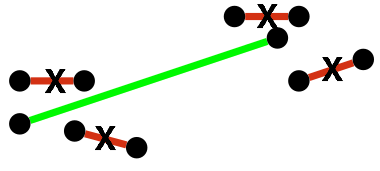
\includegraphics[scale=0.4]{gfx/ConstClust/Inform/Inform} 
	\caption[Informative constraint set.]{Informative constraint set \cite{davidson2007survey}.}\label{fig:Informativity}
\end{figure}


Informativity is estimated using the constraint set as a test set, so the ability of the algorithm to predict the constraints present in it is measured. Formally, given a set of constraints $CS$ and a constrained clustering algorithm $A$, we get the partition $C_A$ by applying the algorithm to the input dataset specifying an empty constraint set. We can compute the number of unsatisfied constraints in $C_A$ a in Equation \ref{eq:Informativity} \cite{davidson2007survey}.

\begin{equation}
I_A(CS) = \frac{1}{|CS|}\left[ \sum_{r \in CS} \text{unsat}(r, C_A) \right].
\label{eq:Informativity}
\end{equation}

\textbf{Coherence} measures the degree of agreement within the set of constraints itself with respect to a given metric. For instance, Figure \ref{fig:Coherence} shows two parallel and very close constraints of different type. It is in cases like this that the contradiction occurs, as the \acs{ML} constraints indicate that the distance between instances involved in them is small, while \acsp{CL} indicate the opposite.

\begin{figure}[!h]
	\centering
	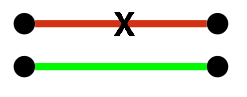
\includegraphics[scale=0.4]{gfx/ConstClust/Coherencia/Coher1}
	\caption[Non-coherent constraint set.]{Non-coherent constraint set \cite{davidson2007survey}.}\label{fig:Coherence}
\end{figure}

Then, the coherence measure is given by the degree of overlap that constraints produce by interpreting them as vectors in space and projecting them along one of the axes, as shown in Figure \ref{fig:CoherenceOverlap}.

\begin{figure}[!h]
	\centering
	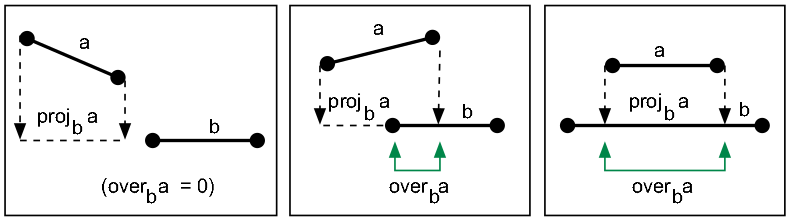
\includegraphics[scale=0.4]{gfx/ConstClust/Coherencia/Coher2}
	\caption[Coherence measure representation.]{Coherence measure representation \cite{davidson2007survey}.}\label{fig:CoherenceOverlap}
\end{figure}

\section{Summary}

Constrained clustering adds a new type of information to the original clustering problem, which is given in the form of specifications of belonging to the same or to different clusters on pairs of instances. Constraints, whether they are the pairwise \acf{ML} and \acf{CL} constraints, or the distance-based $\delta$ and $\epsilon$ constraints, are used to guide the clustering method being applied to a dataset in its search for a result partition that meets certain desired properties.

Clustering methods derived from this concept have proved to be advantageous in many areas; in addition to this, they suffer from some issues that can be tackled by carefully studying the constraints used to solve each individual problem.



	% Backmatter

	%\appendix
	%\renewcommand{\thechapter}{\alph{chapter}}
	%\cleardoublepage
	%\part{Appendix}
	%\include{Chapters/Chapter0A}
	%********************************************************************
	% Other Stuff in the Back
	%*******************************************************
	\cleardoublepage\defbibheading{bibintoc}[\bibname]{%
  \phantomsection
  \manualmark
  \markboth{\spacedlowsmallcaps{#1}}{\spacedlowsmallcaps{#1}}%
  \addtocontents{toc}{\protect\vspace{\beforebibskip}}%
  \addcontentsline{toc}{chapter}{\tocEntry{#1}}%
  \chapter*{#1}%
}
\printbibliography[heading=bibintoc] 

	\cleardoublepage%*******************************************************
% Declaration
%*******************************************************
\refstepcounter{dummy}
\pdfbookmark[0]{Declaration}{declaration}
\chapter*{Declaración de Originalidad}
\thispagestyle{empty}

\bigskip

\noindent \textbf{D. GERMÁN GONZÁLEZ ALMAGRO} con DNI $76593910$T, actuando en su propio nombre y derecho,\\

\noindent \textbf{DECLARA, BAJO SU RESPONSABILIDAD}:\\

\noindent Que el Trabajo Fin de Grado presentado en la Escuela Técnica Superior de Ingenierías Informática y de Telecomunicaciones de la Universidad de  Granada, con fecha 17 de Junio de 2018, titulado <<\textit{Constrained Clustering: New Proposals}>> es original, no es copia de ningún otro trabajo, inédito, y no ha sido difundido por ningún medio, ni presentado anteriormente por quien suscribe o por otra persona.\\



\noindent Y para que así conste a los efectos oportunos, firmo la presente en Granada, a 17 de junio de 2018.



\vspace{3cm}

\smallskip

\begin{flushright}
    \begin{tabular}{m{6cm}}
        \\ \hline
        \centering\textbf{Fdo. \myName} \\
    \end{tabular}
\end{flushright}

	\cleardoublepage\pagestyle{empty}

\hfill

\vfill


\pdfbookmark[0]{Colophon}{colophon}
\section*{Colophon}
This document was typeset using the typographical look-and-feel \texttt{classicthesis} developed by Andr\'e Miede and Ivo Pletikosić.
The style was inspired by Robert Bringhurst's seminal book on typography ``\emph{The Elements of Typographic Style}''.
\texttt{classicthesis} is available for both \LaTeX\ and \mLyX:
\begin{center}
\url{https://bitbucket.org/amiede/classicthesis/}
\end{center}

\bigskip

\noindent\finalVersionString 


\end{document}
